\documentclass[12pt, openany]{report}
\usepackage[utf8]{inputenc}
\usepackage[T1]{fontenc}
\usepackage{amsmath,amsfonts,amssymb}
\usepackage{amssymb}
\usepackage{multicol}
\usepackage[a4paper,left=2.5cm,right=2.5cm,top=2.5cm,bottom=2.5cm]{geometry}
\usepackage[english]{babel}
\usepackage{libertine}
\usepackage{graphicx}
\usepackage{wrapfig}
\usepackage{amsthm}
\usepackage{float}
\usepackage{enumitem}
\usepackage{pythonhighlight}
\usepackage[]{titletoc}
\usepackage{empheq}
\usepackage{titlesec}
\usepackage{mathpazo}
\usepackage{xfrac}
\usepackage{textcomp}
\usepackage{mathtools}
\usepackage{hyperref}
\usepackage{caption}
\usepackage{tabularray}
\usepackage{subcaption}
\usepackage[bottom]{footmisc}
\usepackage{pdfpages}
\usepackage{tabularx}
\usepackage[skins]{tcolorbox}

\theoremstyle{definition}
\newtheorem{thm}{Theorem}[chapter]
\newtheorem{definition}[thm]{Definition}
\newtheorem{exmp}[thm]{Example} 
\newtheorem{lem}[thm]{Lemma}
\newtheorem{crl}[thm]{Corollary}

\titleformat{\chapter}[display]
  {\normalfont\bfseries}{}{0pt}{\Huge}
\newcommand{\hsp}{\hspace{20pt}}
\newcommand{\HRule}{\rule{\linewidth}{0.5mm}}
\newcommand\independent{\protect\mathpalette{\protect\independenT}{\perp}}
\def\independenT#1#2{\mathrel{\rlap{$#1#2$}\mkern2mu{#1#2}}}
\newcommand{\R}{\mathbb{R}}
\newcommand{\C}{\mathbb{C}}
% Define a new tcolorbox style with a red border and transparent interior
\tcbset{
    redbox/.style={
        enhanced,
        colframe=red,
        colback=white,
        boxrule=1pt,
        sharp corners,
        before skip=10pt,
        after skip=10pt,
        box align=center,
        width=\linewidth-2pt, % Adjust the width dynamically
    }
}
\newcommand{\boxedeq}[1]{
\begin{tcolorbox}[redbox]
    \begin{align}
        #1
    \end{align}
\end{tcolorbox}
}

\hbadness=100000
\begin{document}
\begin{titlepage}
    \begin{sffamily}
    \begin{center}
        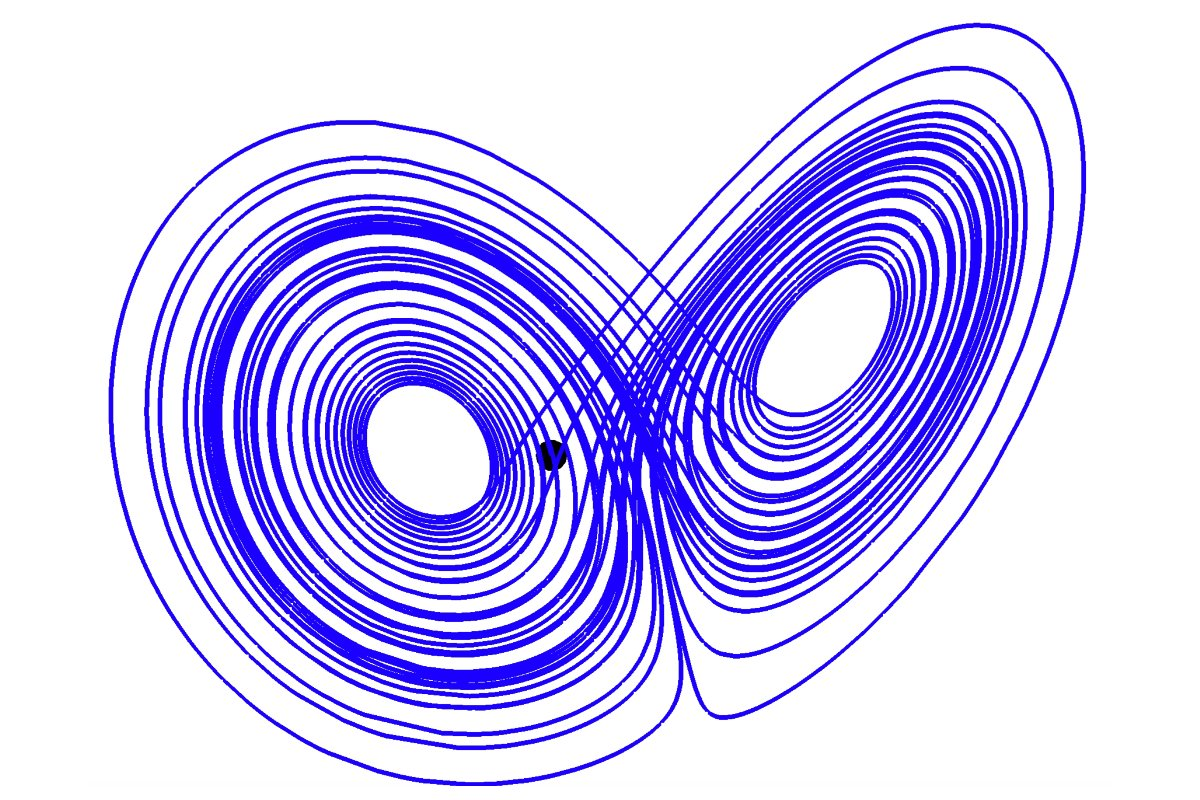
\includegraphics[scale=0.25]{img/page_de_garde.png} \\[1cm]
        \HRule \\[0.4cm]
        { \huge \bfseries LINMA2361 Nonlinear dynamical systems \\[0.4cm] }
    
        \HRule \\[1.5cm]
        \textsc{\LARGE Simon Desmidt}\\[1cm]
        \vfill
        \vspace{2cm}
        {\large Academic year 2024-2025 - Q1}
        \vspace{0.4cm}
         
        
\includegraphics[width=0.15\textwidth]{img/epl.png}
        
        UCLouvain\\
    
    \end{center}
    \end{sffamily}
\end{titlepage}

\setcounter{tocdepth}{1}
\tableofcontents
\chapter{Linear continuous-time 2D dynamical systems}
\section{Introduction}
Consider the 2D dynamical system \(\dot x=f(x),\: x\in \mathbb{R}^n\). Let \(\Omega \subseteq \mathbb{R}^n\) that is compact and positively invariant. Assume that \(f\in \mathcal{C}^1\) on \(\Omega\), i.e. it is continuously differentiable on \(\Omega\). Let \(x(0)\in \Omega\). Then the system has one and only one solution for all positive times. \\

\(\Omega\) is positively invariant if \(x(0)\in \Omega\Longrightarrow x(t)\in \Omega \: \forall t\ge 0\). 
\section{General form}
The general form of a linear dynamical system is 
\begin{equation}
    \dot x=Ax \qquad x\in \mathbb{R}^n
\end{equation}
and its solution is of the form \(x(t) = \exp(At)x(0)\). We will now study the different possibilities of stability, based on the matrix \(A\):
\begin{enumerate}
    \item \(A\) is diagonalizable:
    \begin{enumerate}
        \item \(\lambda_1>\lambda_2>0\) : unstable (repelling) node (see LINMA2370).
        \item \(\lambda_1>\lambda_2=0\) : 
        \item \(\lambda_1>0>\lambda_2\) : saddle point.
        \item \(0=\lambda_1>\lambda_2\) : 
        \item \(0>\lambda_1>\lambda_2\) : attracting node.
        \item \(\lambda_1=\lambda_2>0\) : unstable star, the eigenvectors are perpendicular and the direction is repelling from the origin.
        \item \(\lambda_1=\lambda_2=0\) : every point is an equilibrium.
        \item \(\lambda_1=\lambda_2<0\) : stable star, the eigenvectors are perpendicular and the direction is going to the origin.
    \end{enumerate}
    \item \(A\) has two equal eigenvalues with only one eigenvector, i.e. is not diagonalizable:
    \begin{enumerate}
        \item \(\lambda<0\): convergence to the equilibrium point.
        \item \(\lambda=0\): 
        \item \(\lambda>0\):
    \end{enumerate}
    \item \(A\) has complex conjugate eigenvalues:
    \begin{enumerate}
        \item \(Re(\lambda)>0\): diverges from the equilibrium in a spiral form.
        \item \(Re(\lambda)=0\): the trajectory is periodic, does not converge nor diverge.
        \item \(Re(\lambda)<0\): converges to the equilibrium in a spiral form.
    \end{enumerate}
\end{enumerate}
\chapter{Nonlinear CT, 2D systems}
\section{General form}
The general form of a nonlinear CT 2D dynamical system is 
\begin{equation}
    \dot x = f(x)\qquad x\in \R^2, \: f:\R^2\rightarrow \R^2
\end{equation}
A nullcline is a curve such that for an element \(x_i\) of \(x\), \(\dot x_i=0\). There are two in a 2D system and their intersections are the equilibrium points. The vector field has a horizontal or vertical direction on those curves., and their sense is given by the sign of \(\dot x\) or \(\dot y\).
\begin{itemize}
    \item [\(\rightarrow\)] N.B.: The nullclines cross trajectories, as they are not trajectories themselves. 
\end{itemize}
An equilibrium point is stable if all eigenvalues of the jacobian matrix evaluated at that point have nonpositive real part. It is said to be hyperbolic if its real part is nonzero. 
\begin{thm}
    Consider the initial value problem \(\dot x=f(x),x(0)=x_0\). Suppose that \(f\) is continuous and all its partial derivaties are continuous for \(x\) in some open connected set \(D\subseteq \R^n\). Then for \(x_0\in D\), the initial value problem has a solution \(x(t)\) and the solution is unique. \\
    This means that existence and uniqueness of solutions are guaranteed if \(f\) is continuously differentiable.
\end{thm}
\section{Methodology}
\begin{enumerate}
    \item Nullclines: Find the graph of the functions such that \(\dot x=0\), \(\dot y=0\).
    \item Equilibrium points: Those are the intersections of both nullclines.
    \item Stability: Analyze the eigenvalues of the Jacobian matrix at each equilibrium point.
\end{enumerate}
\section{Linearization}
The system here is 
\begin{align}\label{eq:2D-CT}
    \dot x &= f(x,y)\nonumber \\
    \dot y &= g(x,y)
\end{align}
If \((x^*,y^*)\) is one of its equilibrium points, then the Jacobian matrix for that point is 
\begin{equation}
    A \coloneqq \begin{pmatrix}
        \frac{\partial f}{\partial x} & \frac{\partial f}{\partial y}\\
        \frac{\partial g}{\partial x} & \frac{\partial g}{\partial y}\\
    \end{pmatrix}_{(x^*,y^*)}
\end{equation}
and the linearized system is 
\begin{equation}
    \begin{pmatrix}
        \dot u\\ \dot v
    \end{pmatrix} = A \begin{pmatrix}
        u\\ v
    \end{pmatrix}
\end{equation}
with \(u=x-x^*\) and \(v=y-y^*\). 
\section{Population dynamics}
The Lotka-Volterra model of competition is used to model the population growth of two species fighting for the same finite resources, but not eating each other, e.g. sheeps and rabbits. The state-space model is
\begin{align}
    \dot x &= x(3-x-2y)\nonumber \\
    \dot y &= y(2-y-x)
\end{align}    
Its equilibrium points are \((0,0), (0,2),(3,0),(1,1)\). The first is an unstable node, the next two are stable and the last is a saddle point. 
\begin{figure}[H]
    \centering
    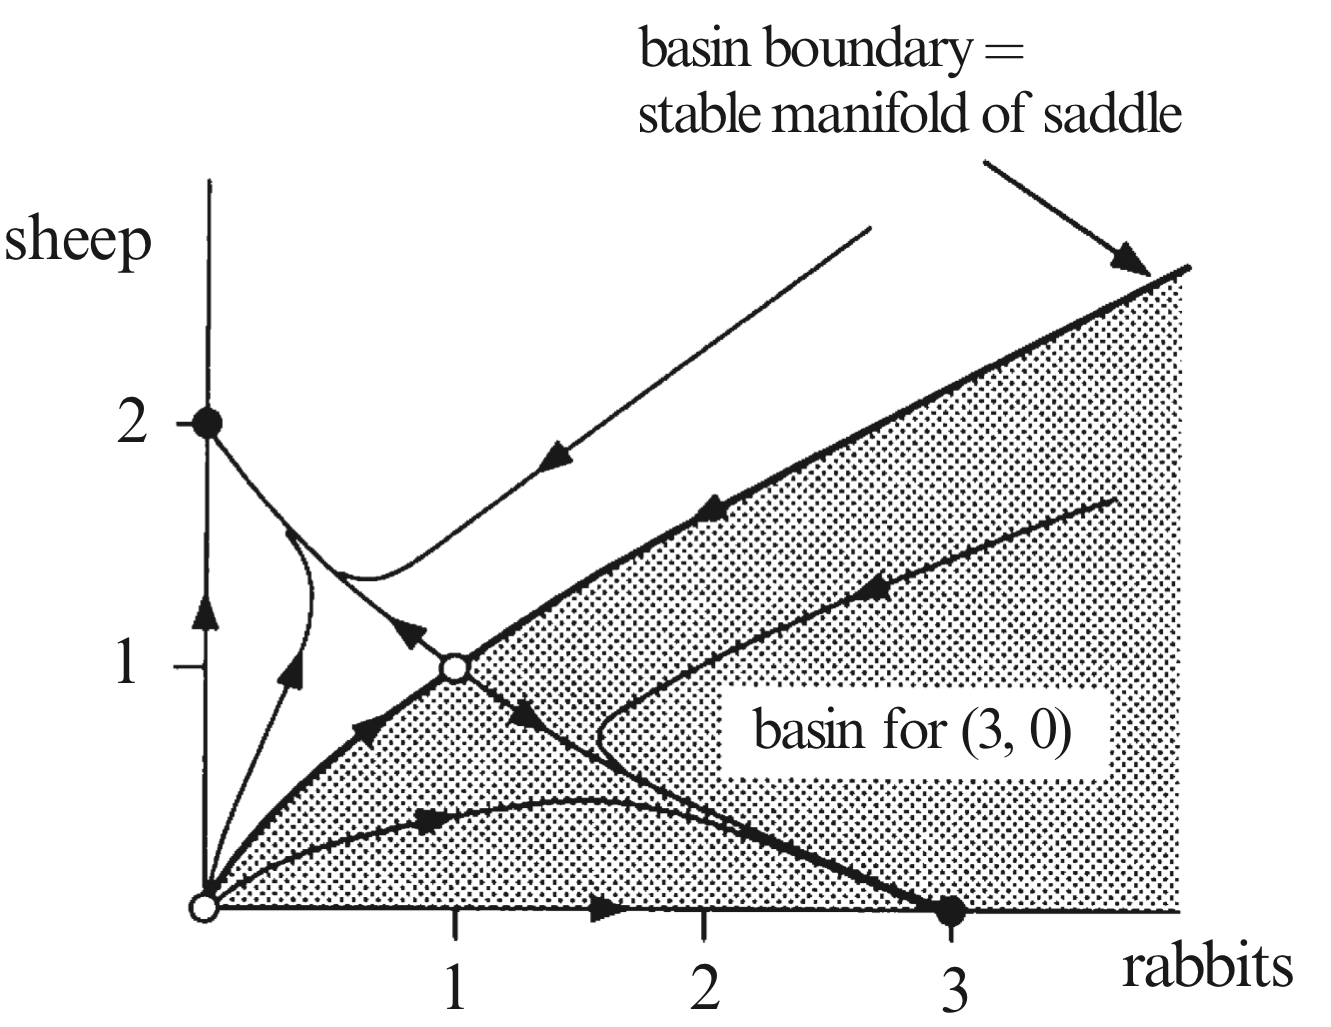
\includegraphics[width = .5\textwidth]{img/basin_of_attraction.png}
\end{figure}
\begin{itemize}
    \item [\(\rightarrow\)] N.B.: the stable manifold is the boundary between the regions of the two stable equilibria. On one side of the stable manifold, evey trajectory converges to one equilibrium, and to the other one on the other side. Due to this characteristic, it is also called the basin boundary. 
    \item [\(\rightarrow\)] N.B.: if the real part of the eigenvalues is zero, additionnal information is needed to conclude on the stability. 
\end{itemize}
\section{Conservative systems}
A conservative system is such that there exists a quantity \(V:\R\rightarrow \R\) such that it is constant, according to the time, along every trajectory. It often has the dimensions of an energy. 
\begin{thm}
    Consider the system \(\dot x=f(x)\), \(x\in \R^2\) and \(f\in \mathcal{C}^1\). Suppose that there exists a conserved quantity \(E(x)\) and suppose that \(x^*\) is an isolated fixed point. If \(x^*\) is a local minimum of \(E\), then all trajectories sufficiently close to \(x^*\) are closed.
\end{thm}
\section{Reversible systems}
\begin{definition}
    If the system \(\begin{cases} \dot x =f(x,y)\\ \dot y=g(x,y) \end{cases}\) has the same equations under the transformation of coordinates 
    \begin{equation}
        \begin{cases}
            \tau \coloneqq -t\\
            X \coloneqq x\\
            Y \coloneqq -y
        \end{cases}
    \end{equation}
    then the system is reversible. In 2D, this is saying that the system is reversible if \(f\) is odd and \(g\) is even. 
\end{definition}
\begin{thm}
    If \((x^*,y^*)\) is an equilibrium point, center for the linearized system, and the system is reversible, then, when close enough to the equilibrium point, all trajectories are closed curves.
\end{thm}
\begin{figure}[H]
    \centering
    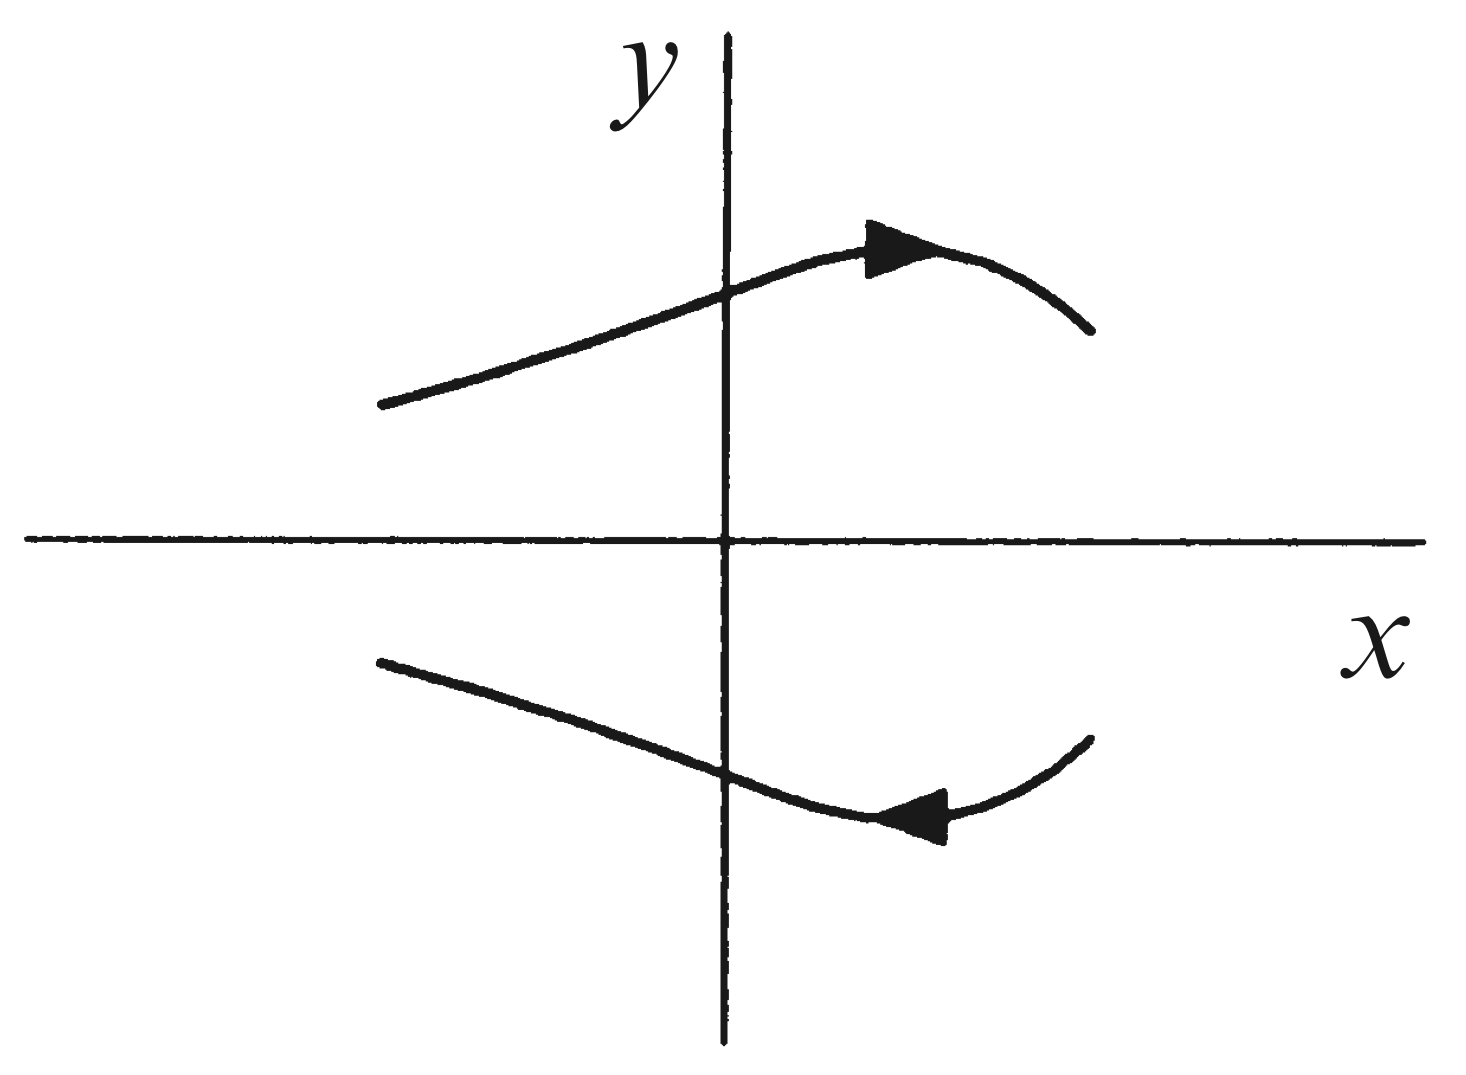
\includegraphics[width = .3\textwidth]{img/reversible.png}
\end{figure}
\begin{itemize}
    \item [\(\rightarrow\)] N.B.: Trajectories that start and end at the same fixed point are called homoclinic orbits. 
\end{itemize}
\section{Invariance principle}
\begin{definition}
    \(x^*\) is a (\(\omega-\))limit point of \(x(t)\) if there exists \(\lim_{t\rightarrow \infty}t_n = \infty\) such that \(\lim_{n\rightarrow \infty}x(t_n)=x^*\).
\end{definition}
\begin{definition}
    A limit set of a trajectory \(x(t)\) is the set of all limit points of that trajectory. It is denoted \(\lim_{\omega}(x(\cdot))\).
\end{definition}
\begin{thm}
    Let the trajectory \(\{x(t);t>0\}\) be bounded. Then, \(\lim_\omega(x(\cdot))\) is nonempty, bounded, closed, invariant and \(\lim_{t\rightarrow \infty}x(t)=\lim_\omega (x(\cdot))\), meaning that the distance between \(x(t)\) and the limit set tends to 0.
\end{thm}
\begin{thm}\textbf{[LaSalle theorem]}
    Let \(V:\R^n\rightarrow \R\), \(V\in \mathcal{C}^1\), such that, \(\dot V(x)\coloneqq \frac{d}{dt}\left(V(\varphi_T(x))\right)_{t=0}\le 0\), \(\forall x\in \R^n\), \(\varphi\) being a mapping such that \(\varphi_T(x(t)) = x(t+T)\). Let us define the sets \(S\coloneqq \{x\in \R^n :\dot V(x)=0\}\) and \(I\) the largest invariant subset of \(S\). Then \(\forall x_0\in \R^n\), \(\lim_\omega (x(\cdot;x_0)) \subseteq I\). Moreover, if \(\{x(t;x_0):t>0\}\) is bounded, then \(\lim_{t\rightarrow \infty}x(t;x_0)=I\). 
\end{thm}
\begin{crl}
    Let \(x^*\) be an equilibrium point of \(\dot x=f(x)\), \(x\in \R^n\). Let \(V:\R^n\rightarrow \R\), \(V\in \mathcal{C}^1\) be positive-definite\footnote{\(V(x^*)=0\), \(V(x)>0\: \forall x\neq x^*\).}. Assume \(\dot V(x)\le 0\) \(\forall x\in \R^n\) and \(S\) is defined as above. Assume that no solution trajectory stays in \(S\) except \(x(t)=x^*\). Then, \(x^*\) is asymptotically stable. 
\end{crl}
\begin{exmp}
    Let us consider the spring-damper system \(\ddot x=-g(x)-h(\dot x)\). where \(g,h\) are gloablly Lipschitz and verifying
    \begin{itemize}
        \item \(g(0)=0\), \(yg(y)>0\) \(\forall y\neq 0, y\in (-a,a)\);
        \item \(h(0)=0\), \(yh(y)>0\) \(\forall y\neq 0, y\in (-a,a)\);
    \end{itemize}
    Then, the origin is a stable equilibrium point. 
\end{exmp}
\section{Index theory}
Let us consider the 2D system \(\dot x=f(x)\), \(x\in \R^2\) and \(f:\R^2\rightarrow \R^2\), \(f\in \mathcal{C}^0\). Let \(C\) be a Jordan curve, i.e. a loop that is continuous and not self intersecting\footnote{Not necessarily a trajectory.}.
\begin{definition}
    The index of \(C\) for \(f\) \(I_C(f)\) is defined as the number of loops that \(f(C)\) does around the origin, counting positive for CCW and negative for CW.
\end{definition}
\begin{itemize}
    \item If \(C_1,C_2\) contain the same fixed points, i.e. we can continuously deform \(C_1\) into \(C_2\) without passing through a fixed point, there indices are equal.
    \item If a Jordan curve contains no fixed point, its index is zero.
    \item The change of variable \(t\rightarrow -t\) does not change the index.
    \item If \(C\) is a trajectory or an orbit for the system, then \(I_C(f) = +1\).
    \item For any Jordan curve \(C\), \(I_C(f) = I_C(-f)\).
\end{itemize}
The index of an isolated equilibrium point \(x^*\) is \(I_{x^*}(f)\coloneqq I_C(f)\), \(C\) being any Jordan curve taken close enought to \(x^*\) to have no other equilibrium point inside. 
\begin{itemize}
    \item For any $C$, $I_C(f)=\sum_i I_{x_i^*}(f)$, $x_i^*$ being the equilibrium points of the system. 
\end{itemize}
\chapter{Bifurcations}
We study here bifurcations in 1 dimension and continuous time. A bifurcation is the evolution of the equilibrium points of the system with a parameter $r$. The system is 
\begin{equation}
    \dot x= f_r(x),\: x\in \R
\end{equation}
and we study the three cases \(r>r_c\), $r=r_c$ and $r<r_c$, $r_c$ being the critical value. 
\section{Saddle-node bifurcation}
The normal form of a system with saddle-node bifurcation is 
\begin{equation}
    \dot x = r+x^2 \eqcolon f_r(x)
\end{equation}
It is the Taylor-developped, shifted and scaled general form.
\begin{figure}[H]
    \centering
    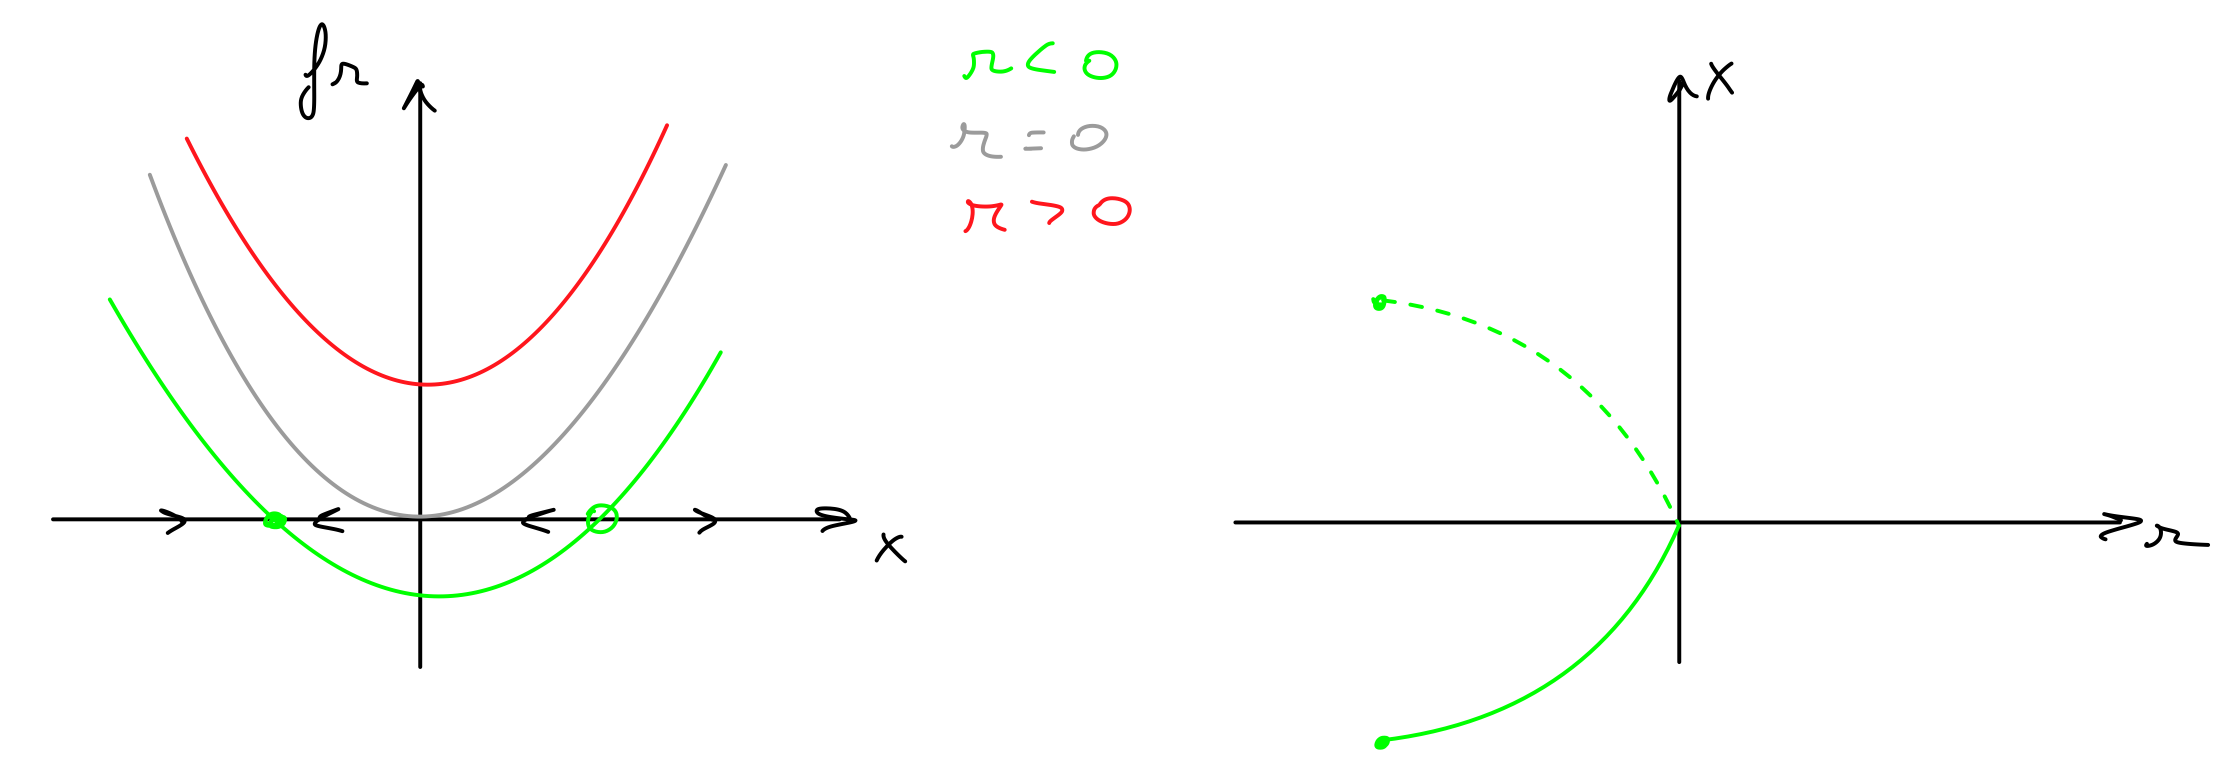
\includegraphics[width=.5\textwidth]{img/saddle_node_bif.png}
\end{figure}
For $r>r_c$, there is no equilibrium point. For $r=r_c$, we have one single equilibrium point, and for $r<r_c$, we have one stable and one unstable equilibrium point. The conditions for this bifurcation to appear are
\begin{align}
    f_{r_c}(x^*)&=0\nonumber\\
    \partial_x f_{r_c}(x^*)&=0\nonumber\\
    \partial_r f_{(r_c)}(x^*)&\neq 0\\
    \partial^2_{xx} f_{r_c}(x^*)&\neq 0\nonumber
\end{align}
\section{Transcritical bifurcation}
The normal form for this case is 
\begin{equation}
    \dot x= rx-x^2\eqcolon f_r(x)
\end{equation}
\begin{figure}[H]
    \centering
    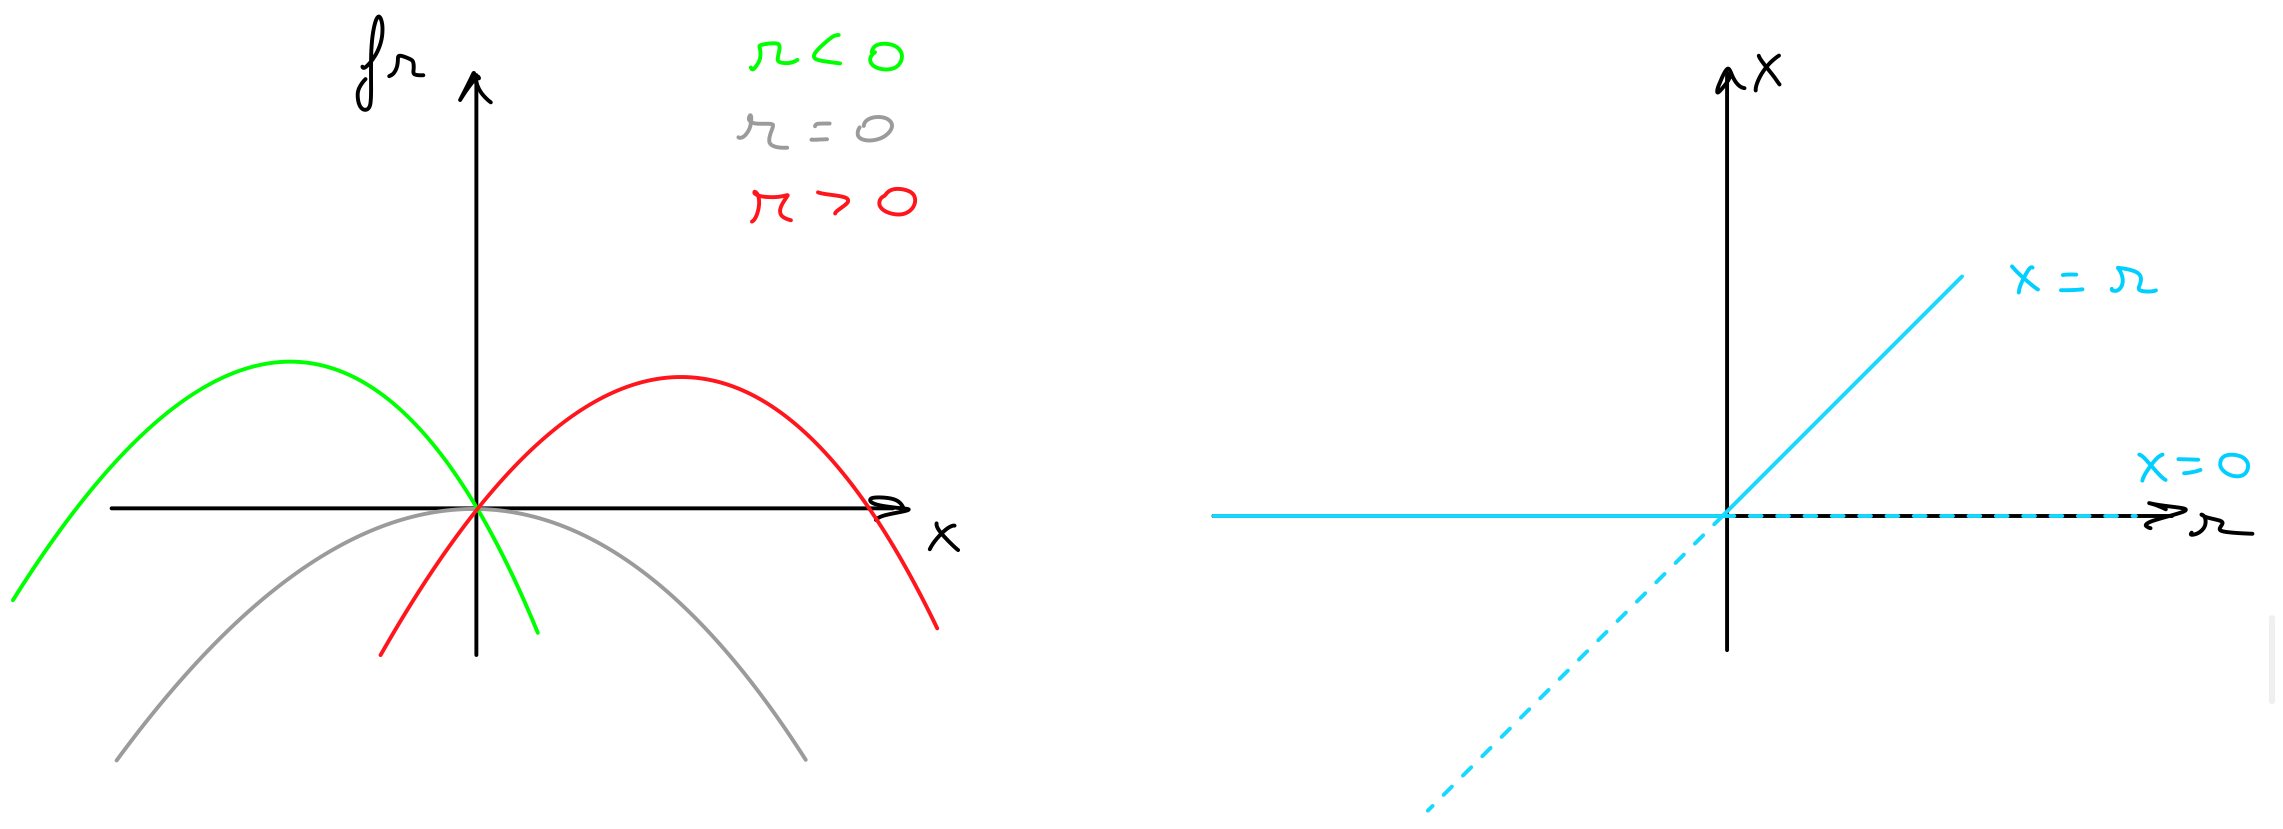
\includegraphics[width = .5\textwidth]{img/transcritical_bif.png}
\end{figure}
At the critical value, the equilibrium points merge and exchange stability. 
\section{Pitchfork bifurcation}
A pitchfork bifurcation often occurs in physical problems that have a symmetry. 
\subsection{Supercritical bifurcation}
The normal form of this bifurcation is 
\begin{equation}
    \dot x = rx-x^3\eqcolon f_r(x)
\end{equation}
\begin{figure}[H]
    \centering
    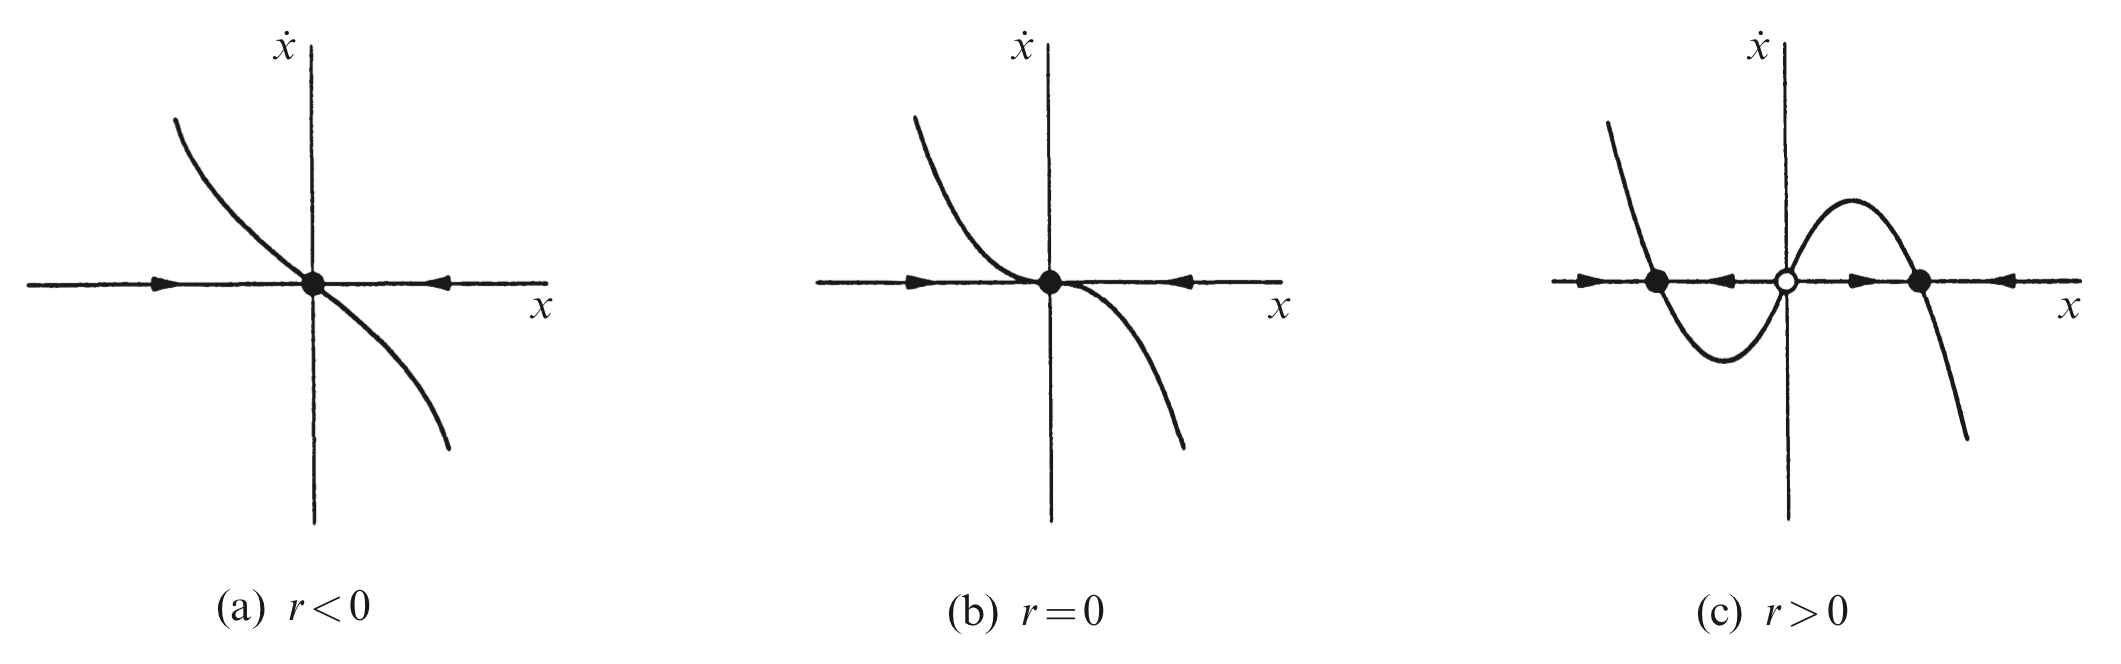
\includegraphics[width = .5\textwidth]{img/pitchfork_bif.png}
\end{figure}
\begin{figure}[H]
    \centering
    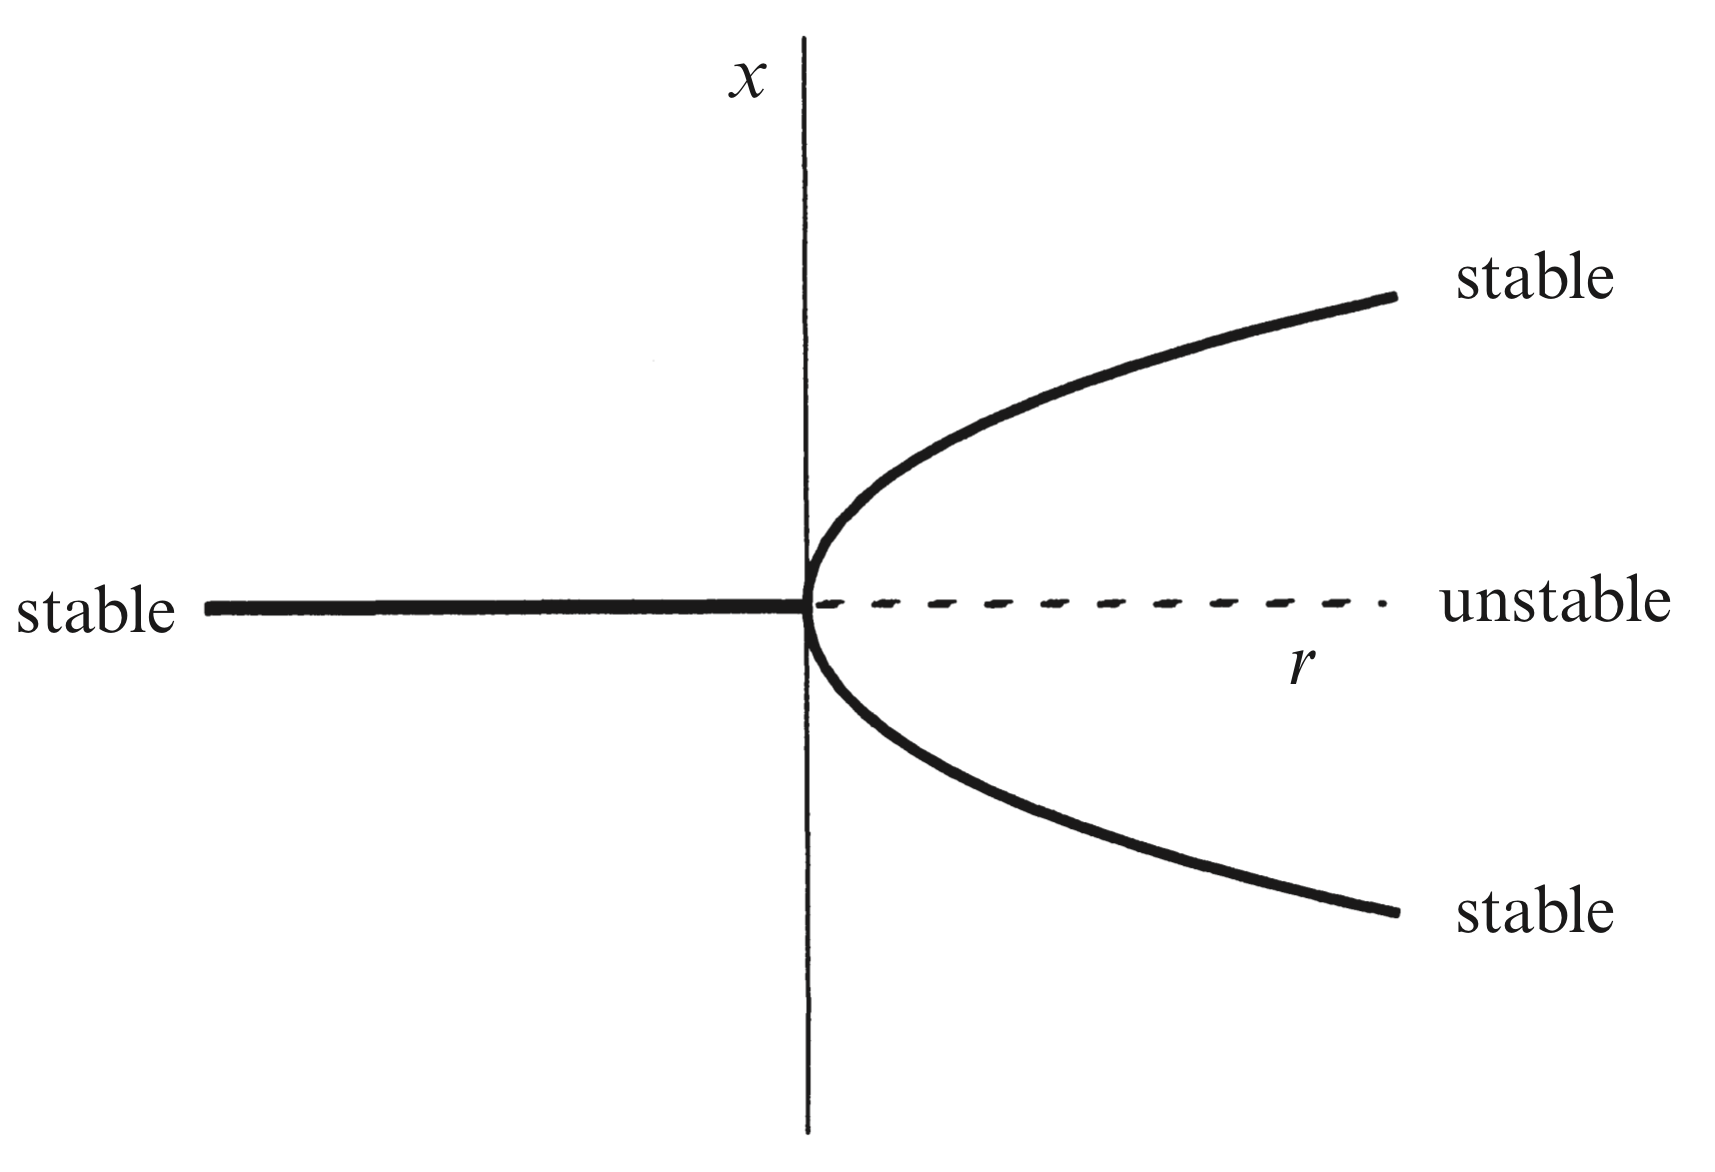
\includegraphics[width = .5\textwidth]{img/supercritical.png}
\end{figure}
There are three stable branches and one unstable.
\subsection{Subcritical bifurcation}
In the subcritical case, there are three unstable branches and one stable. This is however not physically possible and we thus add a $x^5$ term so that the system does not tend to infinity. The canonical form is
\begin{figure}[H]
    \centering
    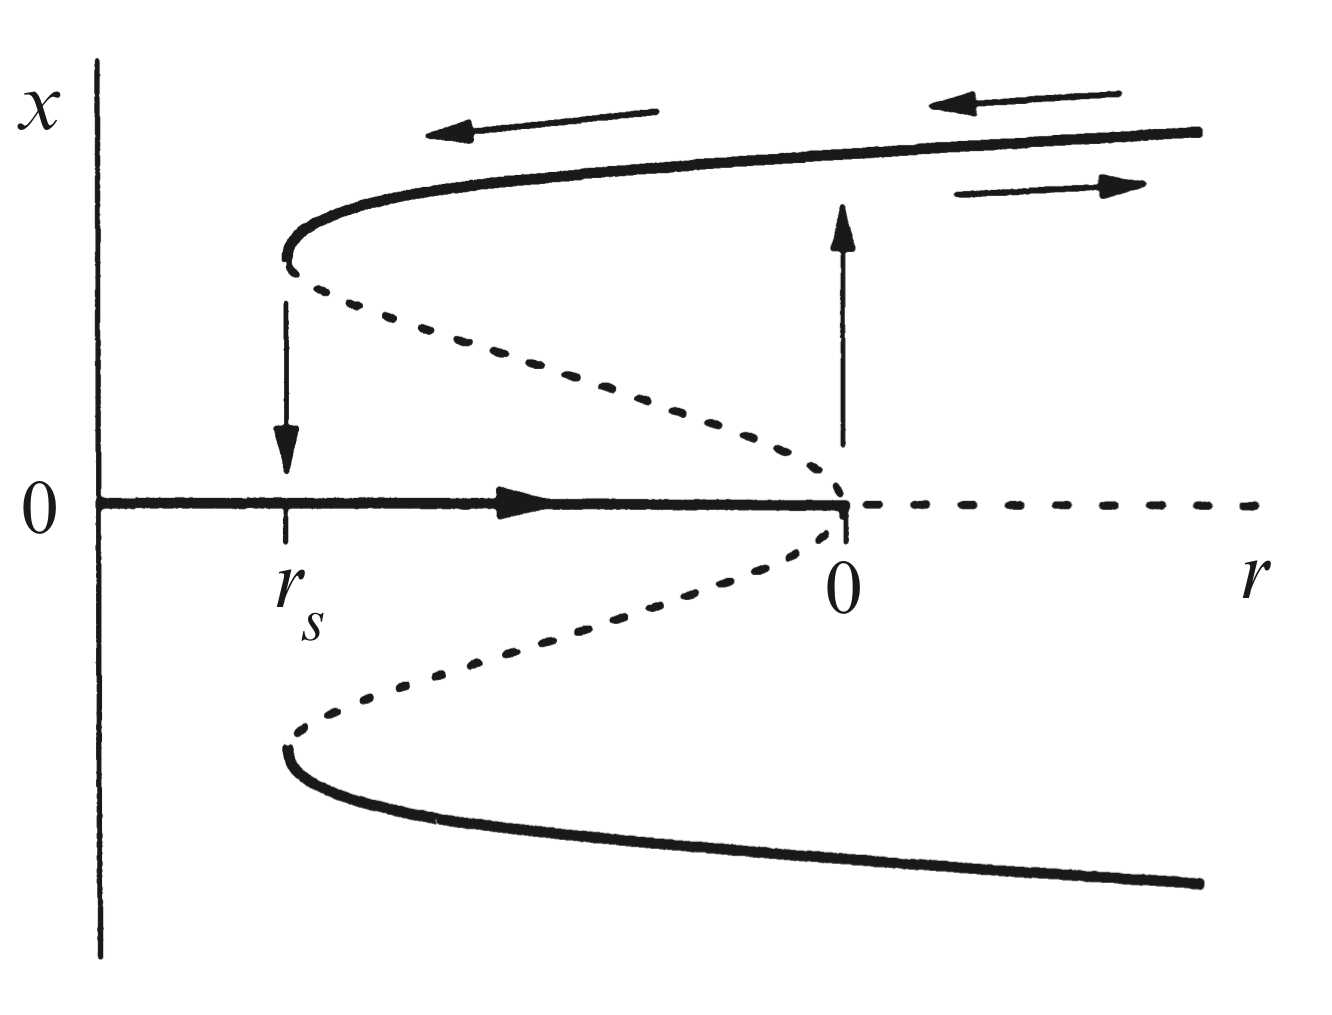
\includegraphics[width = .5\textwidth]{img/subcritical.png}
\end{figure}
\begin{itemize}
    \item In the range $r_s<r<0$, two stable states coexist, and it is the inition condition that determines which fixed point is approach when $t\rightarrow \infty$. That means that the origin is stable under small perturbations, but not big ones (local stability vs global stability). 
    \item The jump between stable curves is called a hysteresis. 
    \item The bifurcation at $r=r_s$ is a saddle-node bifurcation. 
\end{itemize}
\section{Imperfect bifurcations and catastrophes}
Let us here study the system $\dot x= h+rx-x^3$, where $h$ is an imperfection parameter, because it destroys the symmetry of the problem when $h=0$. The fixed points of this system are the intersections of $y=rx-x^3$ and $y=-h$. 
\begin{figure}[H]
    \centering
    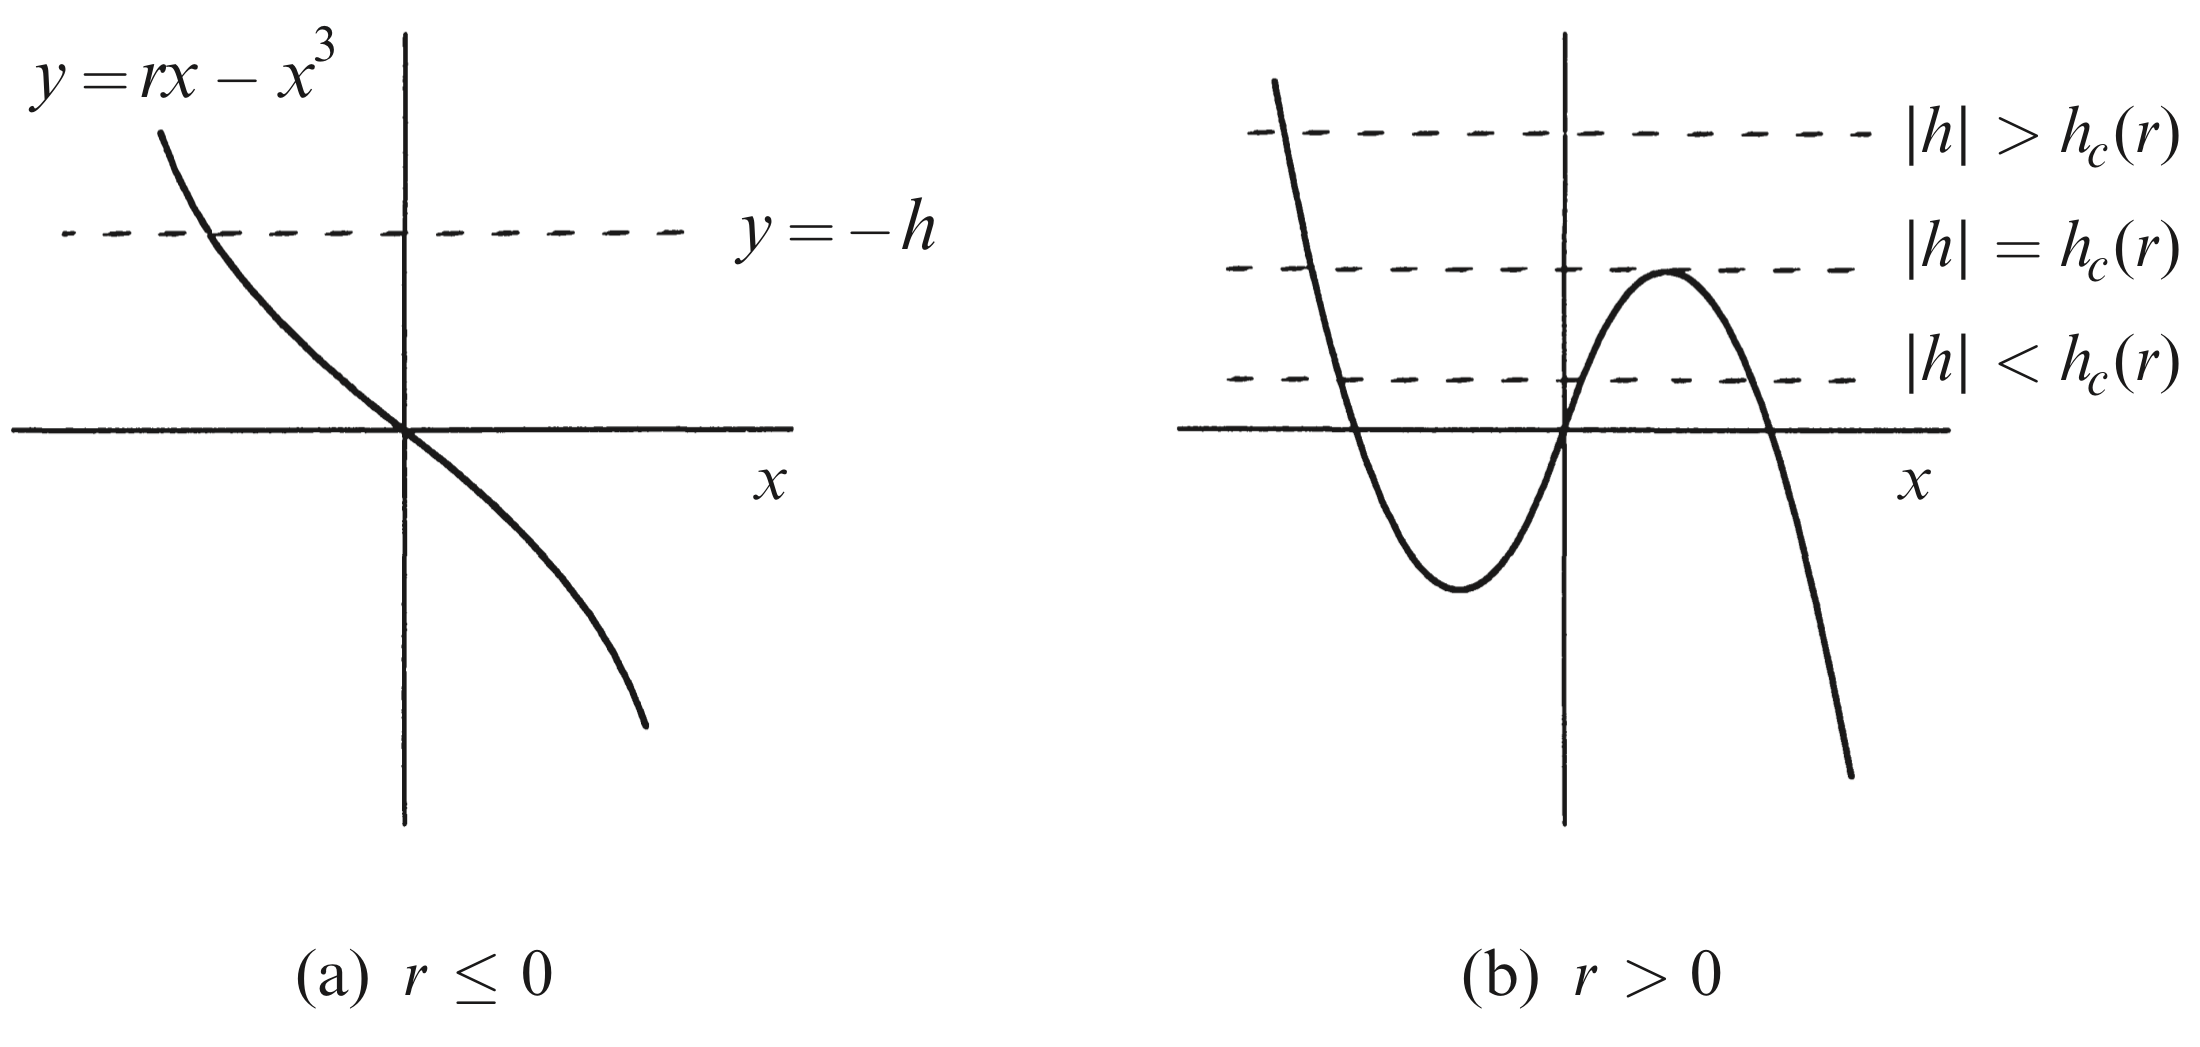
\includegraphics[width = .6\textwidth]{img/saddle_node_impft.png}
\end{figure}
The case $r\le 0$ is not very interesting. For $r>0$, there is a saddle-node bifurcation in $|h| = h_c(r)$, i.e. two bifurcations. The bifurcation curves meet tangentially at $(r,h)= (0,0)$, that point being called a cusp point. 
\begin{figure}[H]
    \centering
    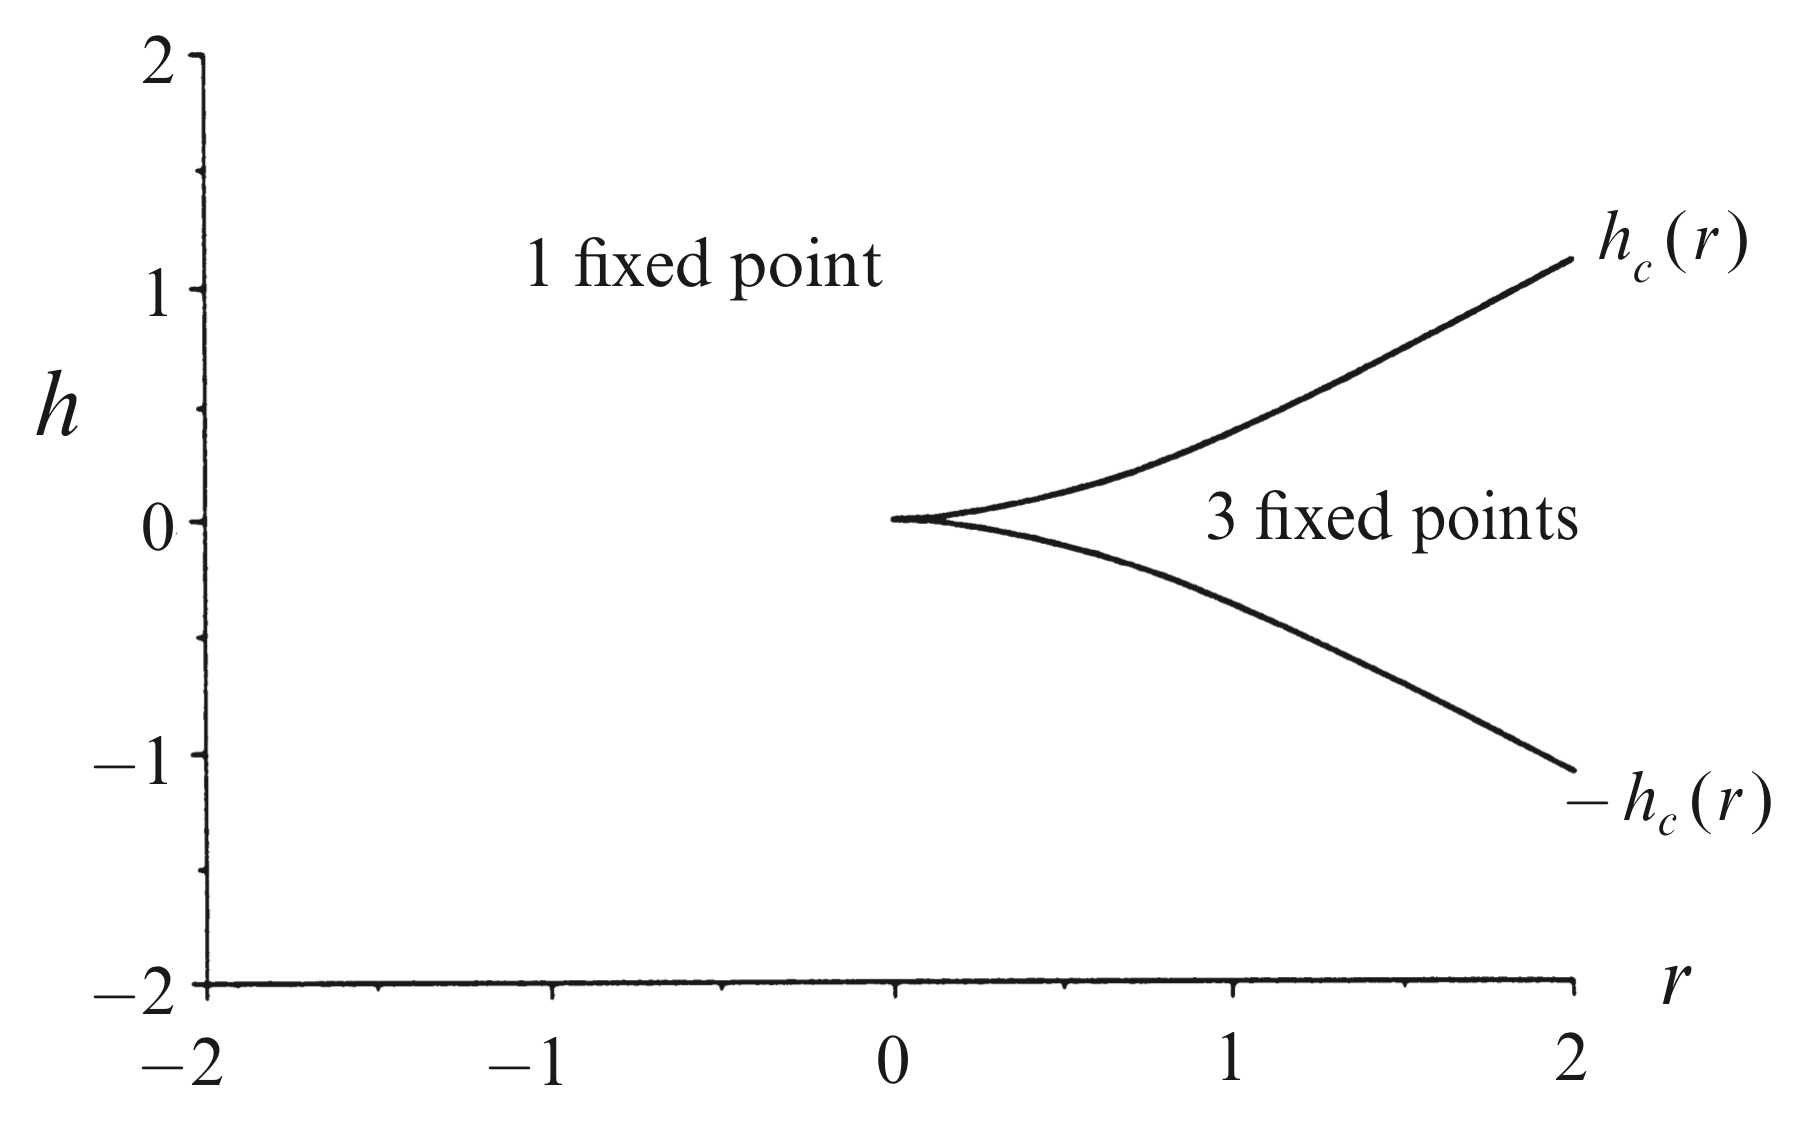
\includegraphics[width=.5\textwidth]{img/cusp.png}
\end{figure}
Let us analyse the behaviour when each of the parameter is changed:
\begin{figure}[H]
    \centering
    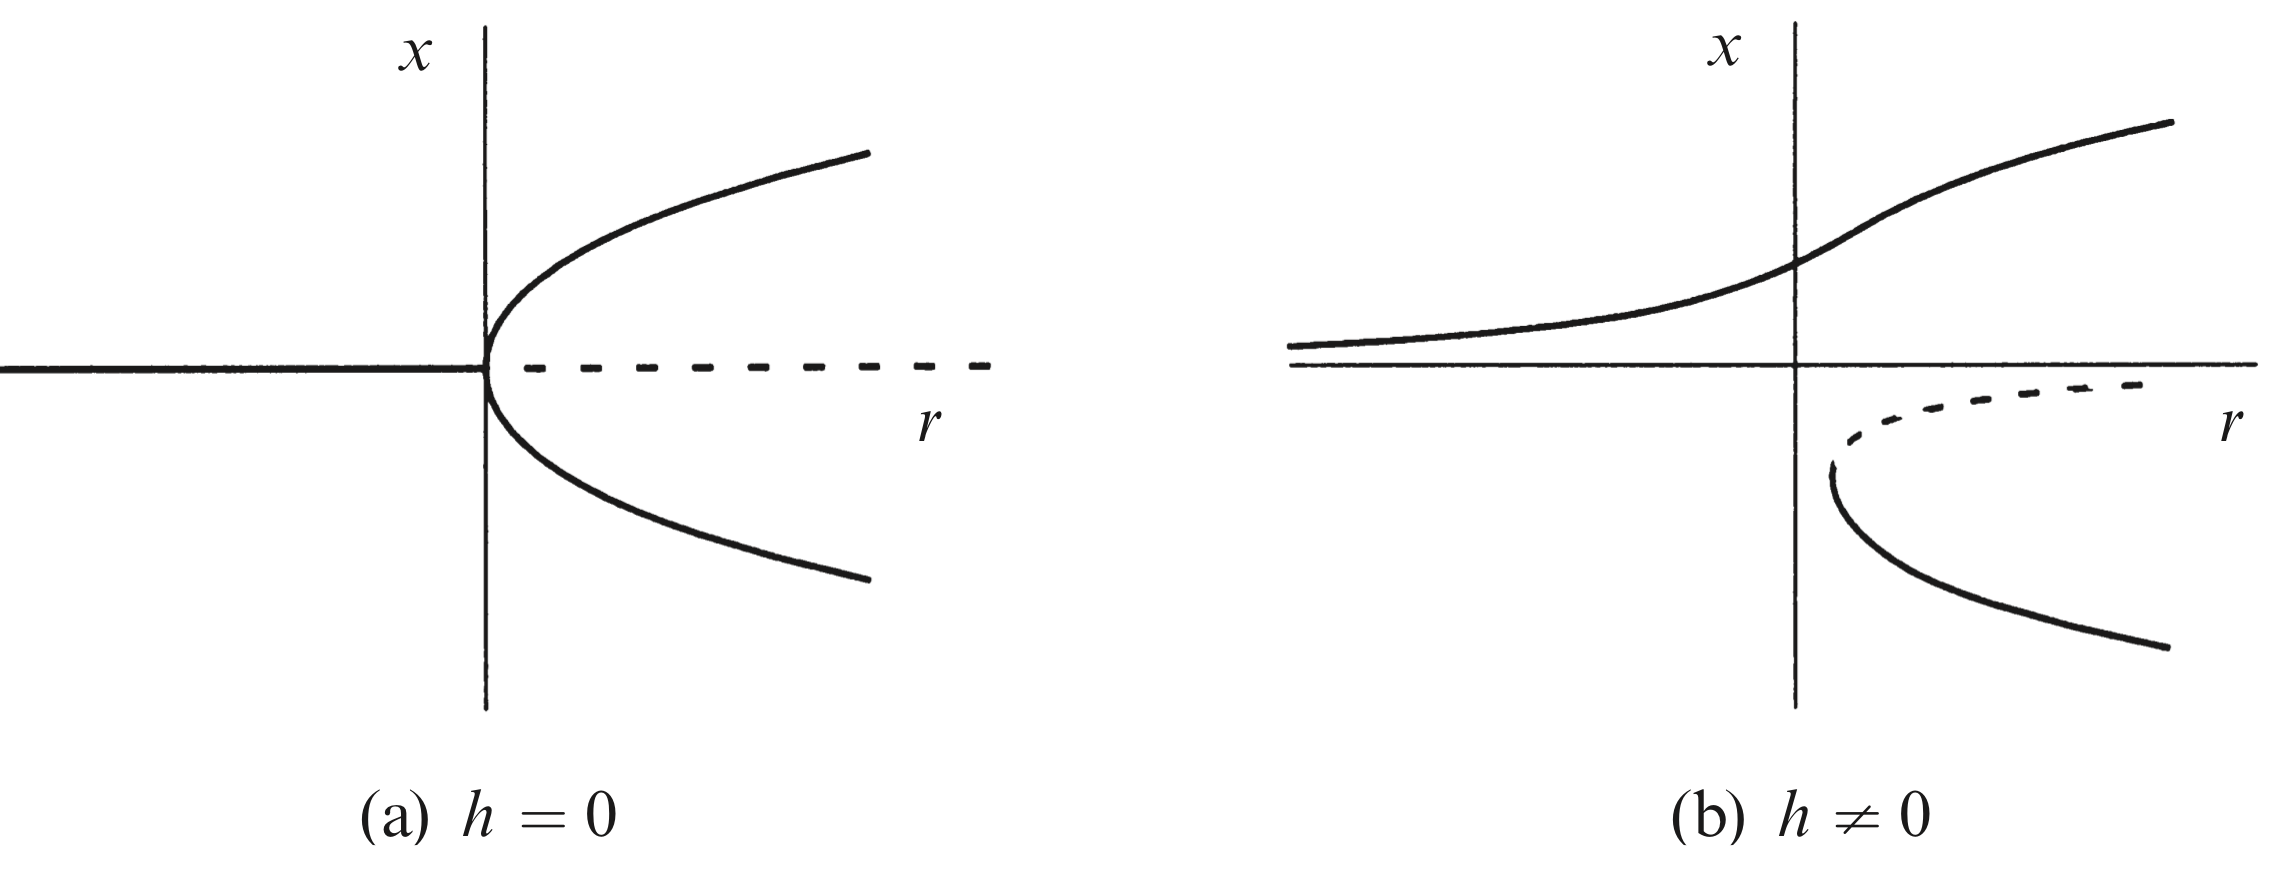
\includegraphics[width=.5\textwidth]{img/h_analysis.png}
\end{figure}
When $h=0$, we have a pitchfork diagram. When $h\neq 0$, the pitchfork disconnects into two pieces, one entirely stable, and the other has a stable and an unstable branch.This means that the lower branch of stable points is not accessible unless we make a fairly large disturbance.
\begin{figure}[H]
    \centering
    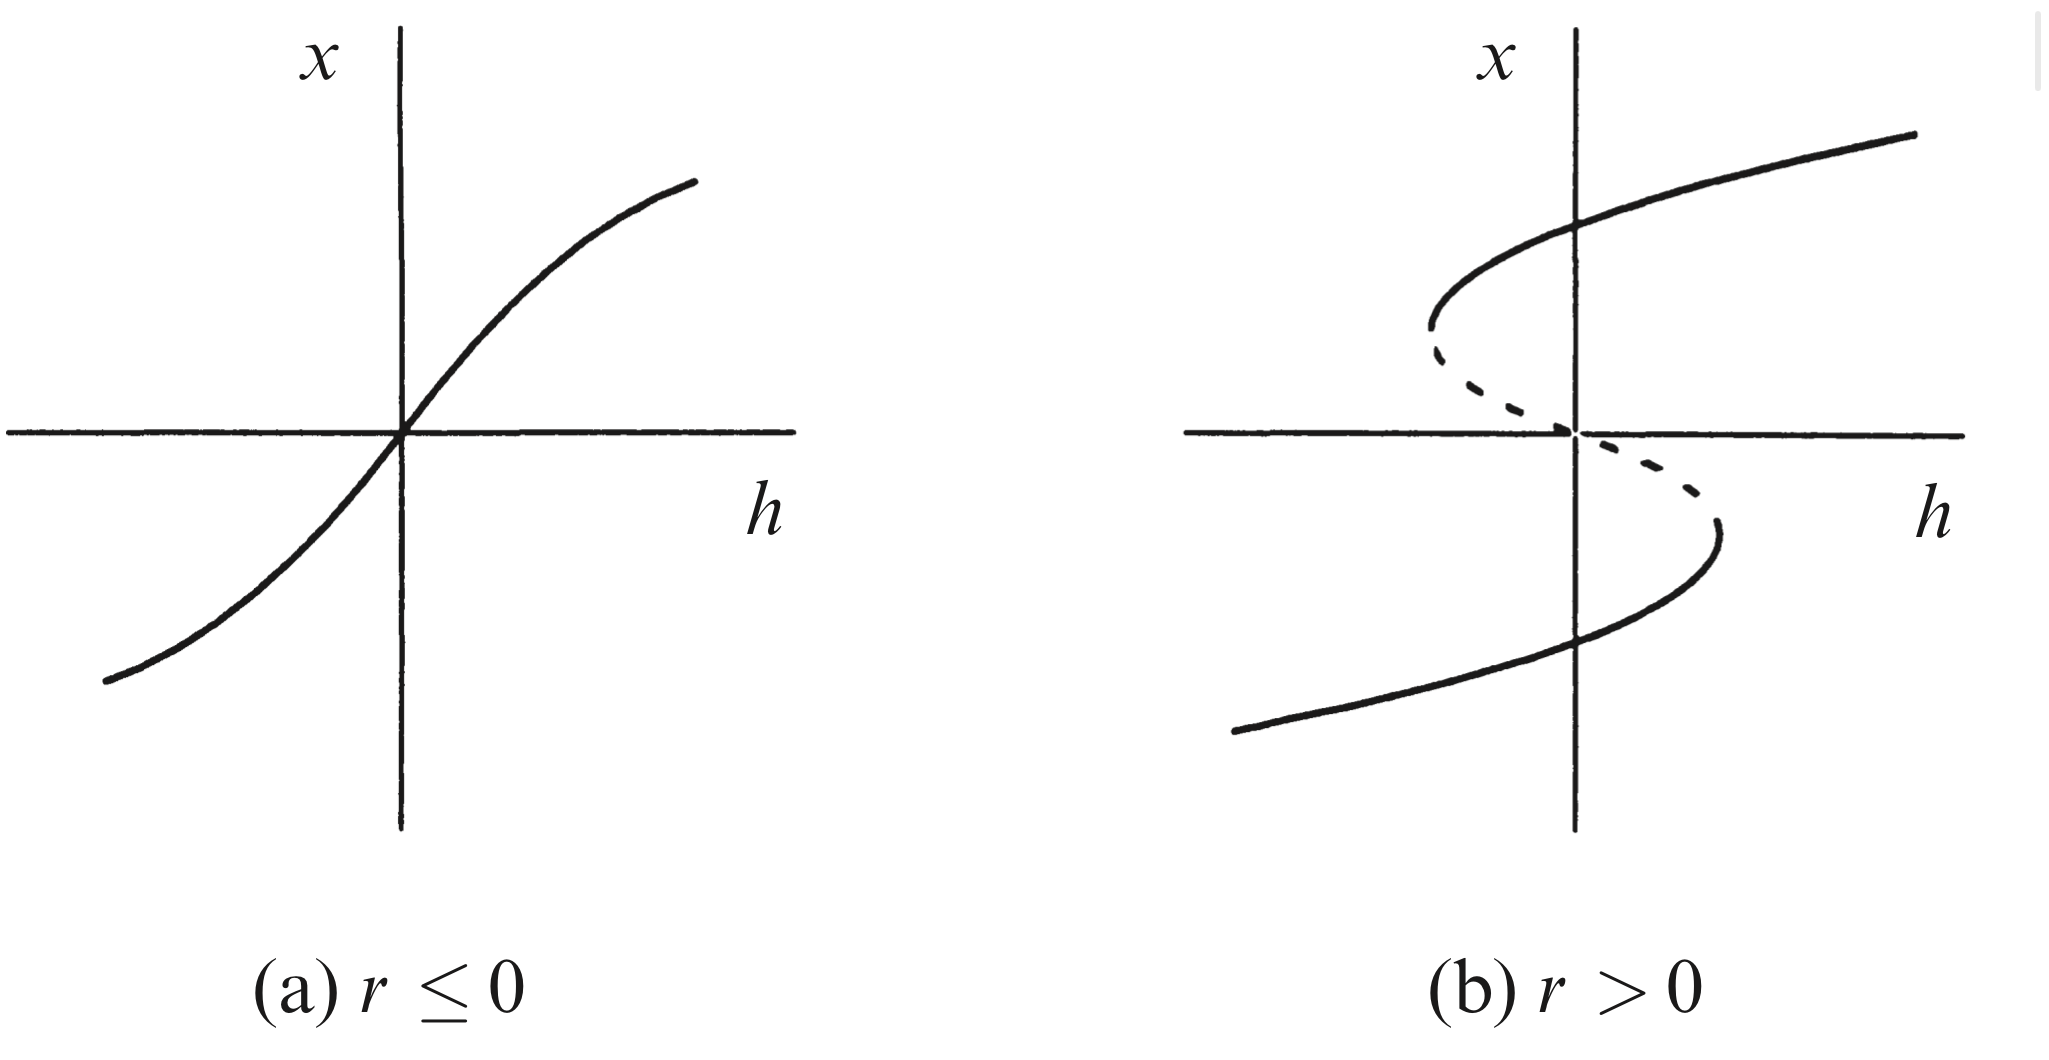
\includegraphics[width=.5\textwidth]{img/r_analysis.png}
\end{figure}
When $r\le 0$, there is one stable point for each $h$. When $r>0$, there are three fixed points when $|h|<h_c(r)$ and one otherwise. \\
In 3D, that gives 
\begin{figure}[H]
    \centering
    \begin{subfigure}[b]{0.49\textwidth}
        \centering
        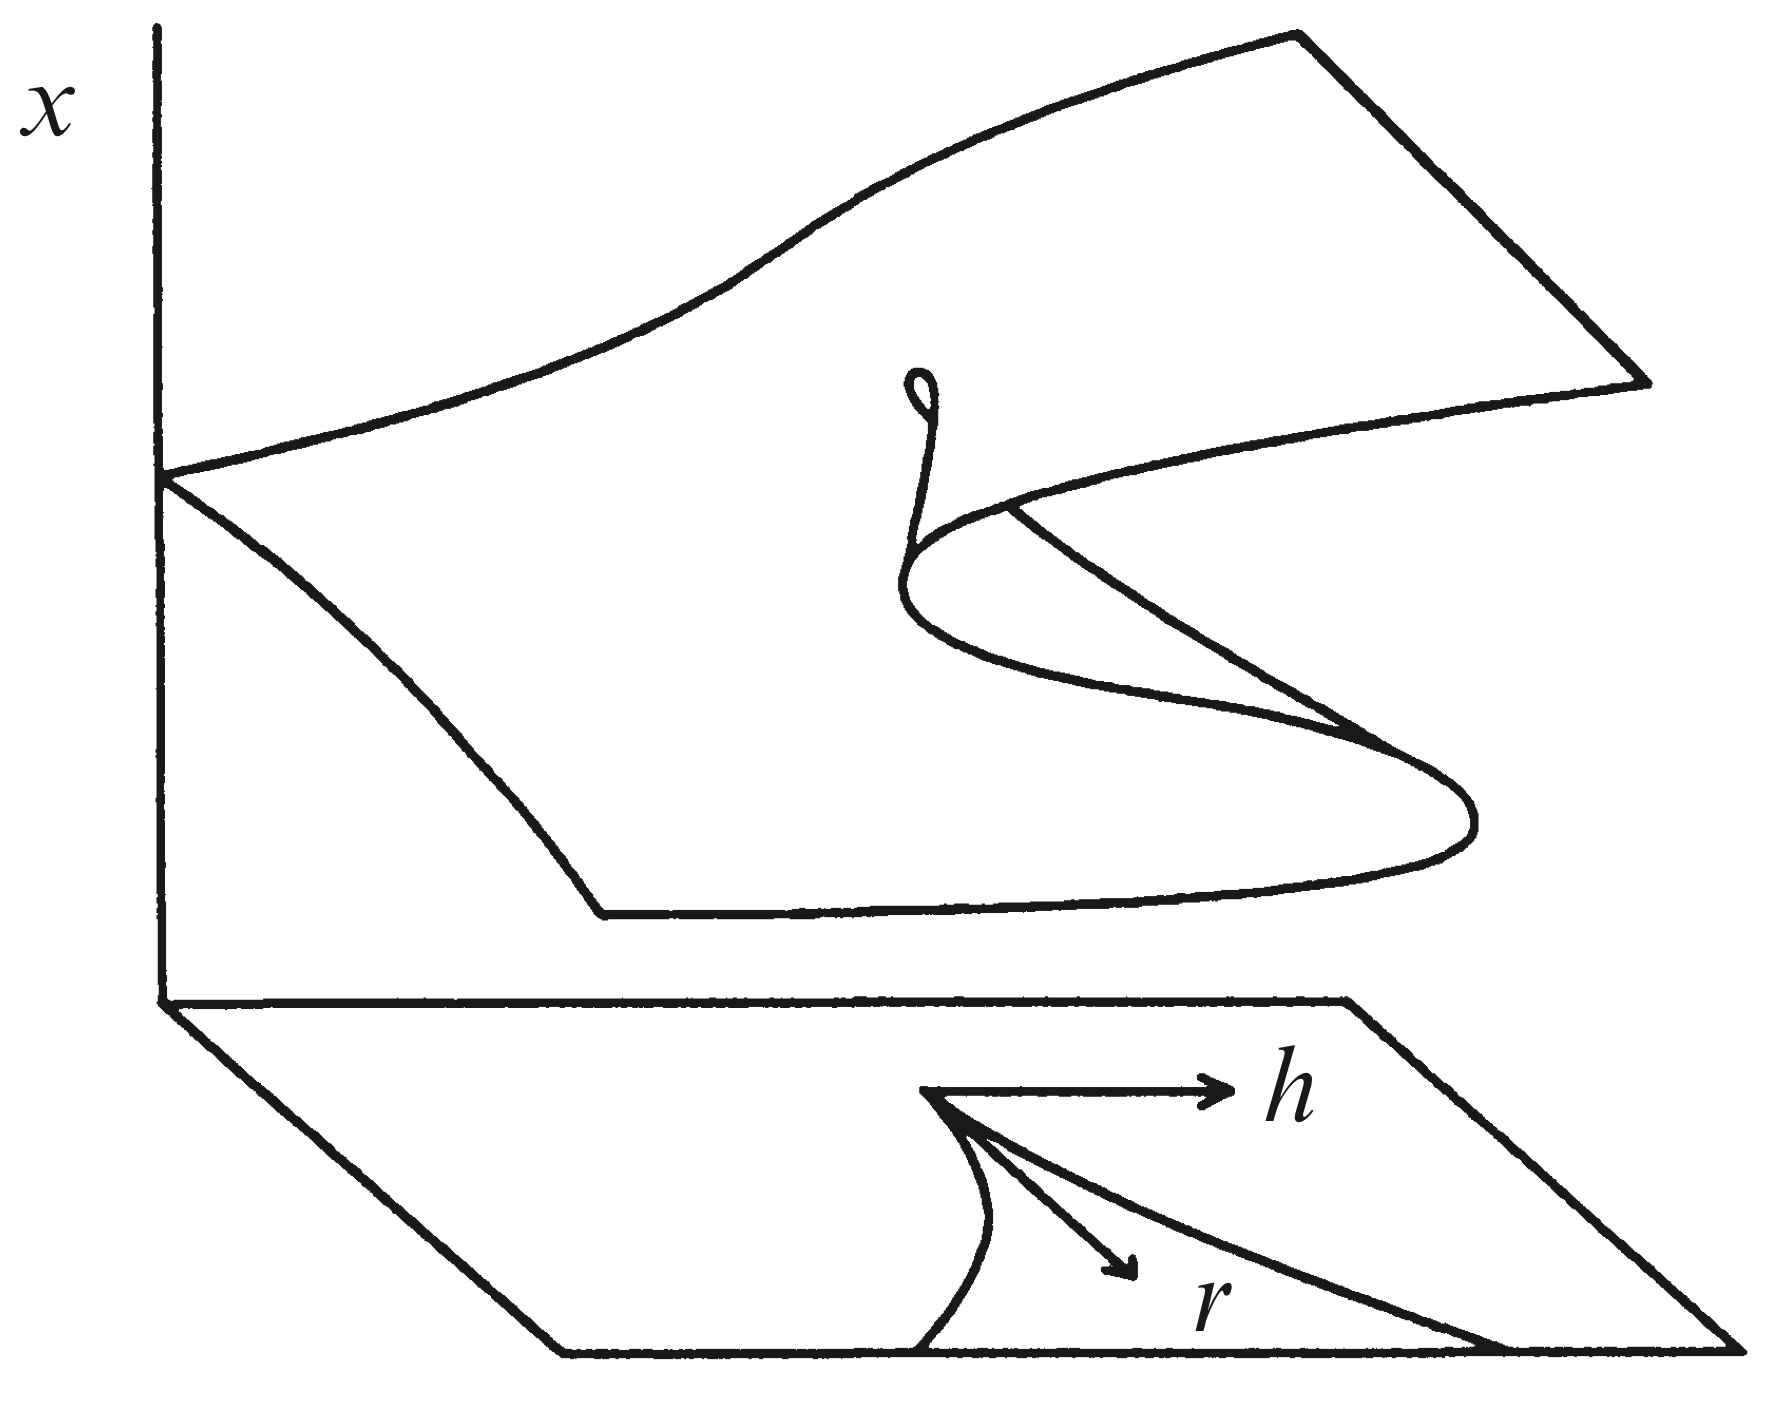
\includegraphics[width=\textwidth]{img/cusp_cata.png}
    \end{subfigure}
    \begin{subfigure}[b]{0.5\textwidth}
        \centering
        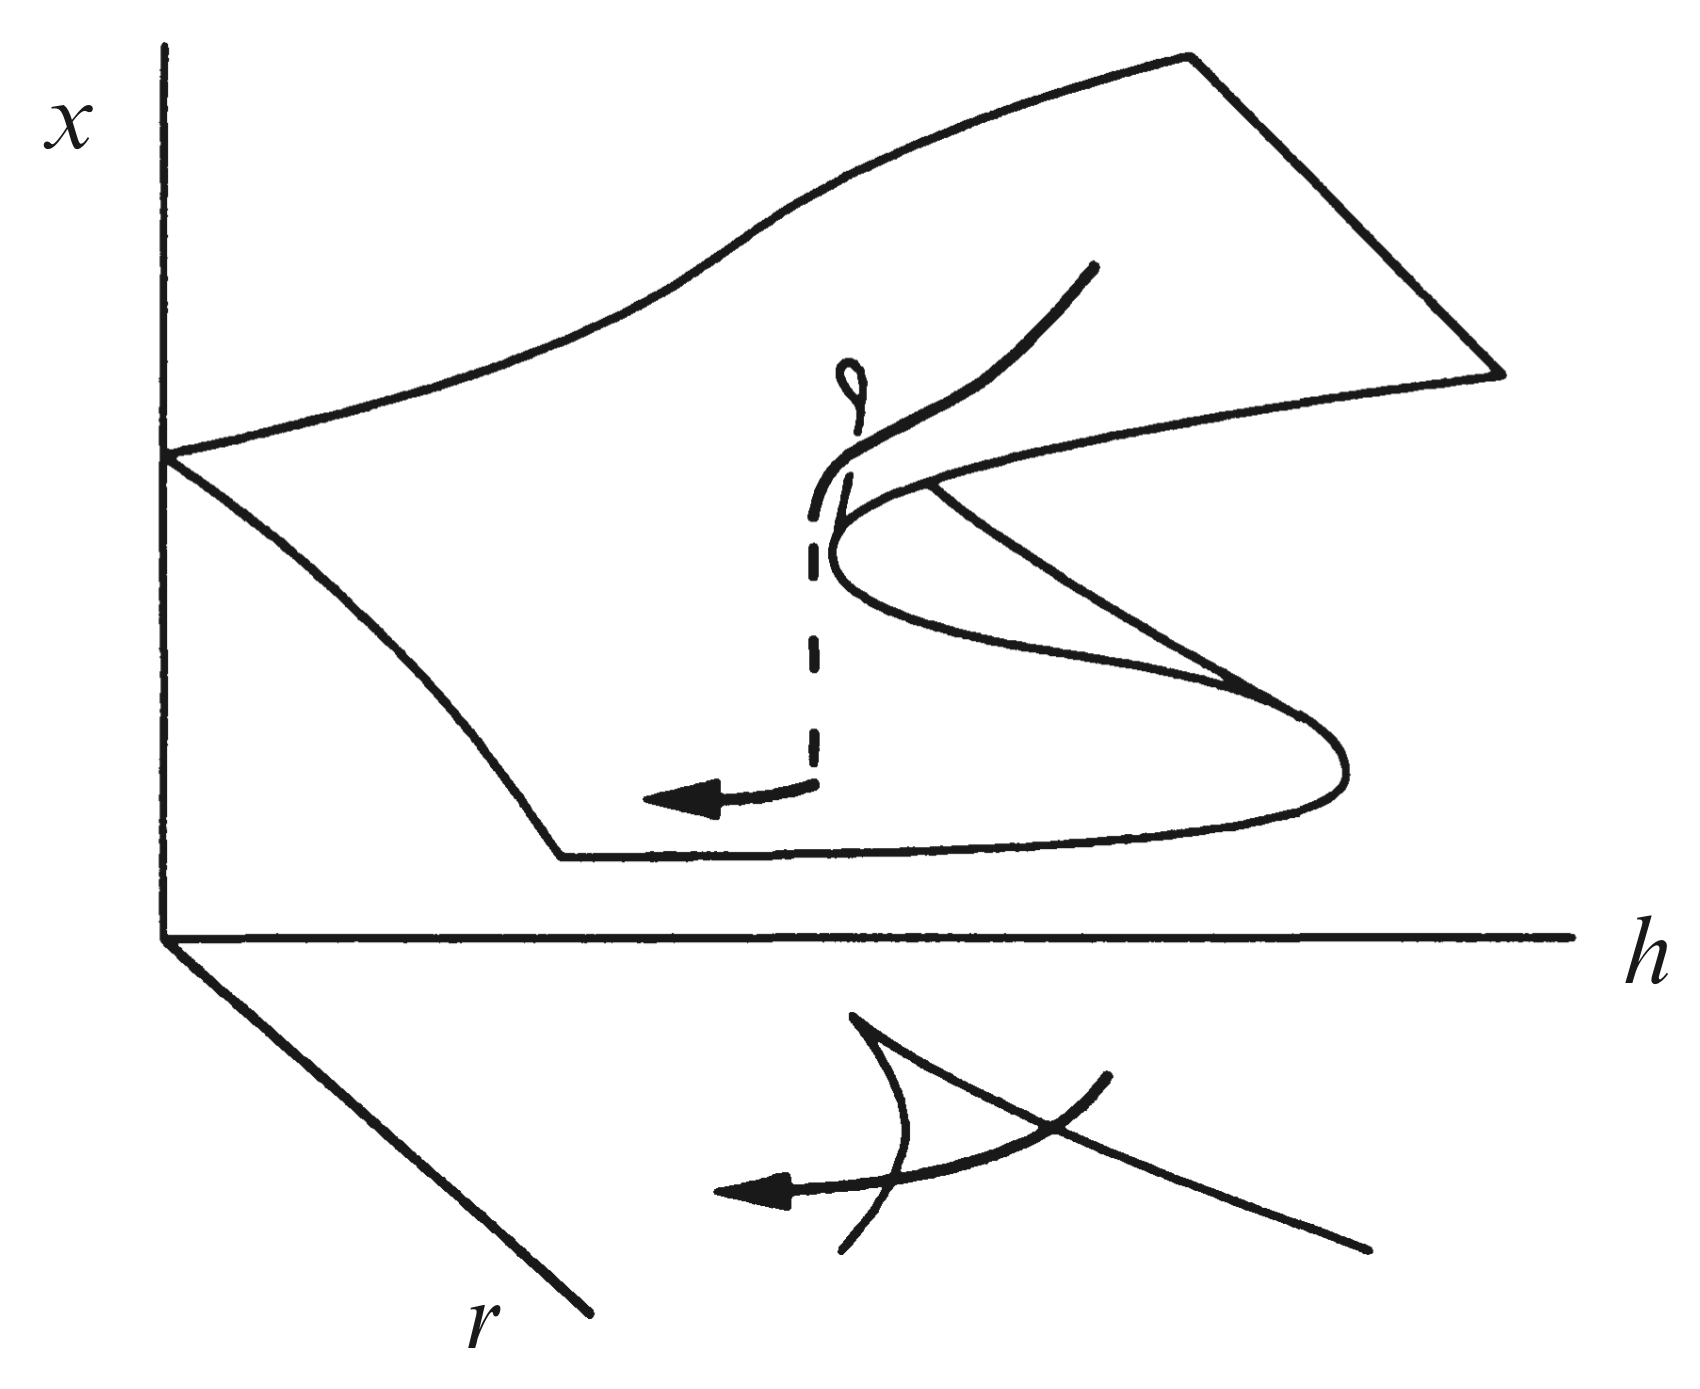
\includegraphics[width=\textwidth]{img/cusp_cata_2.png}
    \end{subfigure}
\end{figure}
and the projection on each plane gives the graphs displayed previously. 
\subsection{Insect outbreak}
This section is an example with the population of insects in a forest. The population model is 
\begin{equation}
    \dot N = RN\left(1-\frac{N}{K}\right) -p(N)\qquad p(N) = \frac{BN^2}{A^2+N^2}
\end{equation}
with $N(t)$ the population, $K$ the growth rate and $K$ the carrying capacity. $p(N)$ is the death rate due to predation of birds. 
\begin{figure}[H]
    \centering
    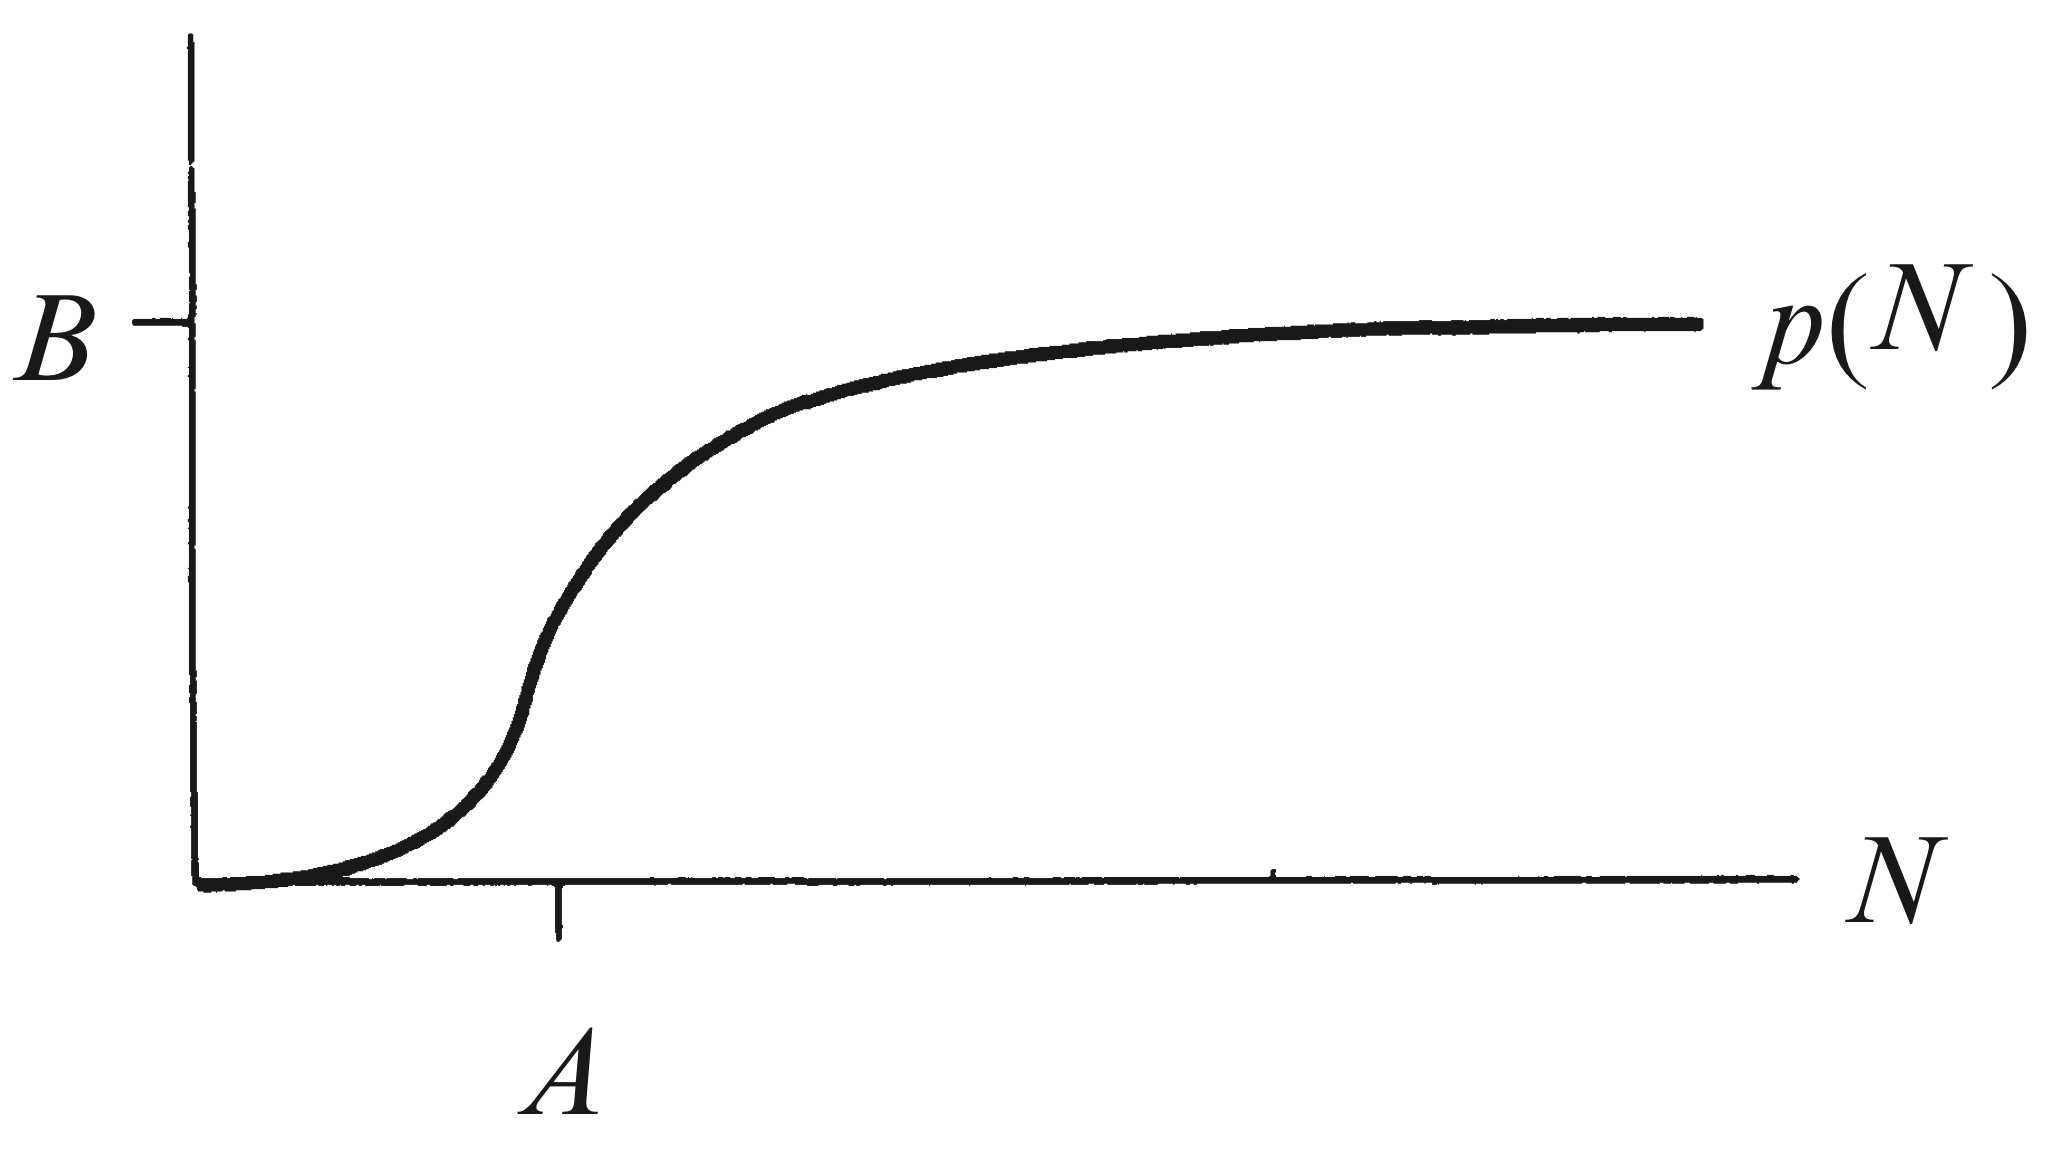
\includegraphics[width = .3\textwidth]{img/predation.png}
\end{figure}
Introducing the adimensionalisation:
\begin{equation}
    x=N/A \qquad \tau = Bt/A \qquad r=RA/B\qquad k=K/A
\end{equation}
the model becomes
\begin{equation}
    \frac{dx}{d\tau}=rx\left(1- \frac{x}{k}\right)-\frac{x^2}{1+x^2}
\end{equation}
$x^*=0$ is always an unstable fixed point, while the others are the solutions of 
\begin{equation}
    r\left(1-\frac{x}{k}\right) = \frac{x}{1+x^2}
\end{equation}
\begin{figure}[H]
    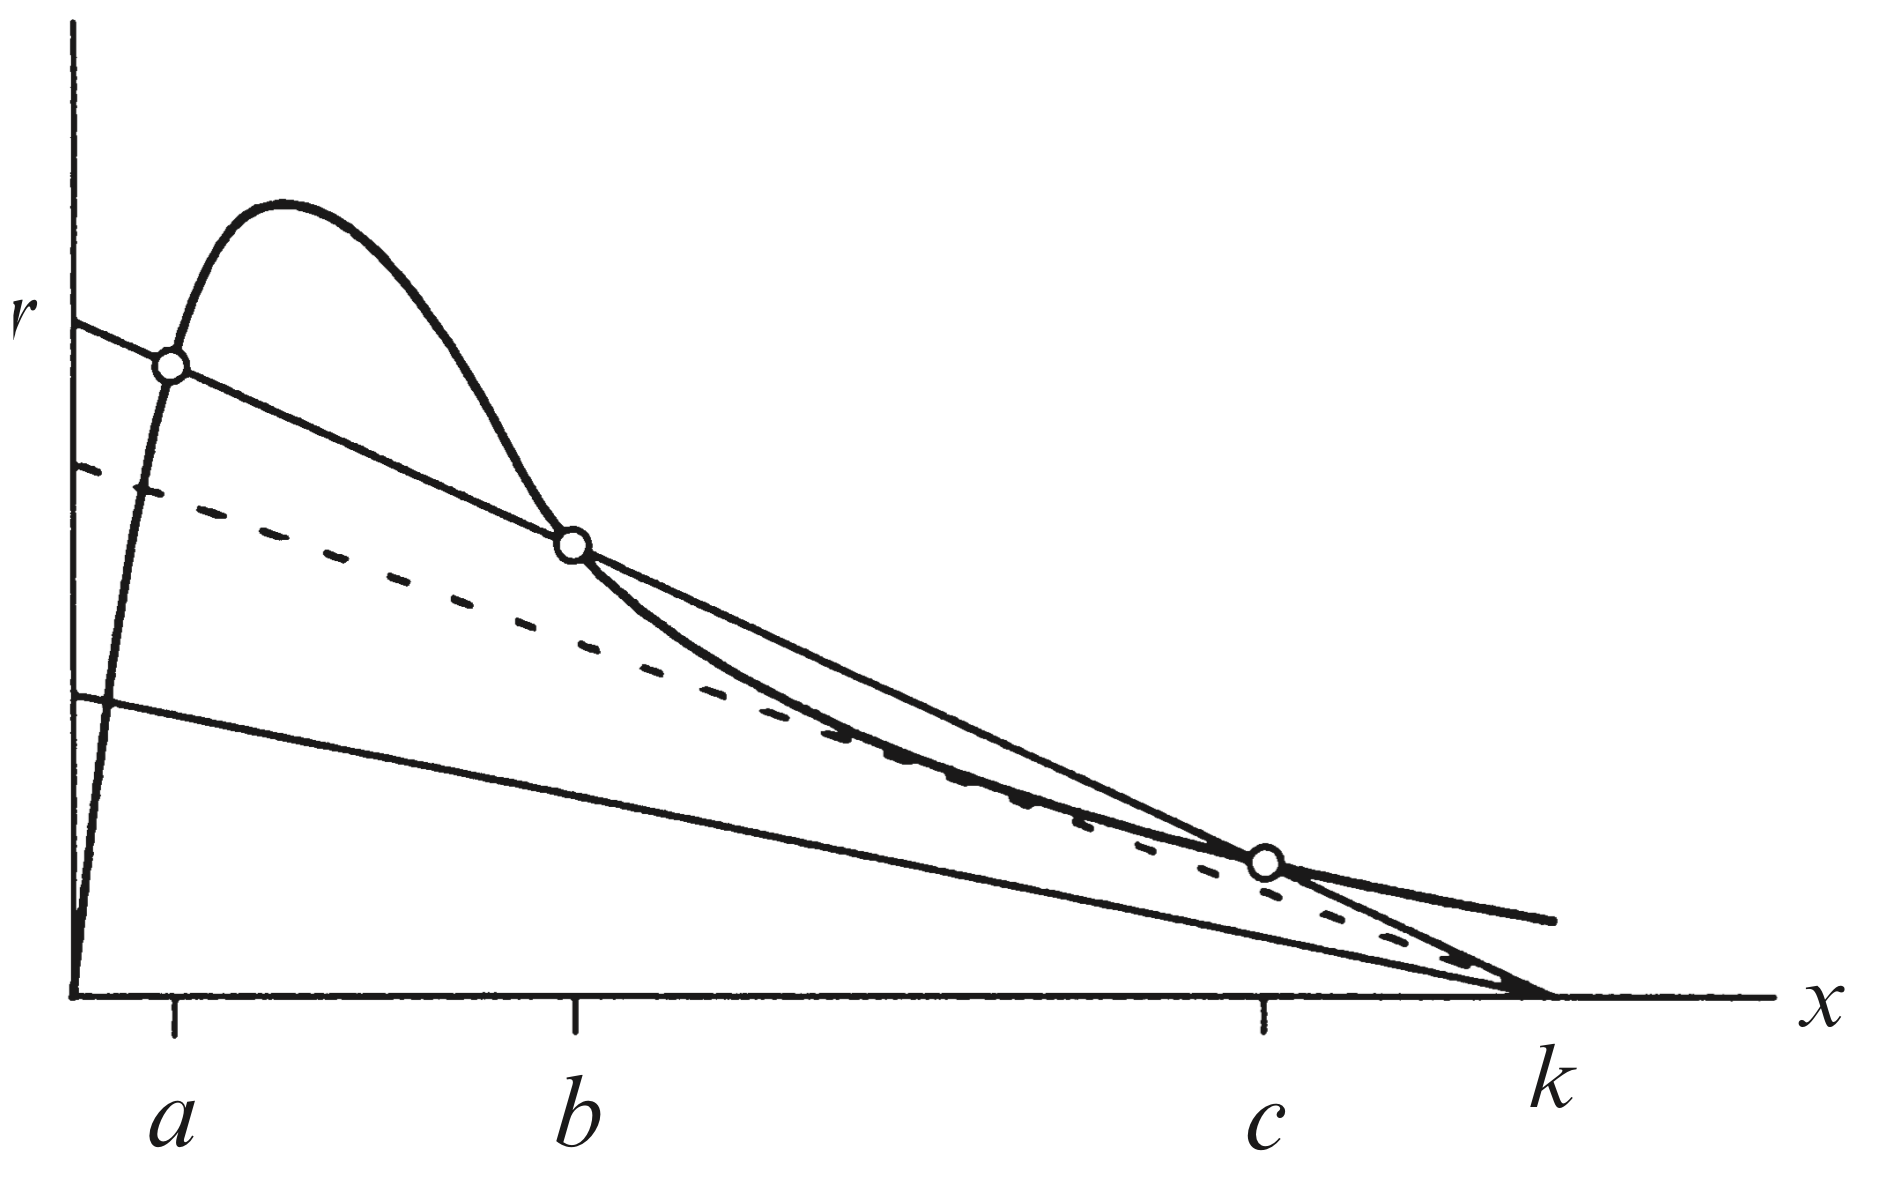
\includegraphics[width=.4\textwidth]{img/budworm.png}
\end{figure}
If $k$ is sufficiently small, there is exactly one intersection for any $r>0$. However, for large $k$, we can have 1, 2, 3 intersections, depending on $r$. As we decrease $r$ with $k$ fixed, the fixed points $b$ and $c$ approach each other and eventually coalesce ina  saddle-node bifurcation when the line intersects the curve tangentially (dashed). After the bifurcation, the only remaining fixed point is $a$. Similarly, $a$ and $b$ can collide and annihilate as $r$ is increased. \\
As the stability type must alternate and 0 is unstable, $a$ and $c$ are stable and $b$ is not. $a$ is called the refuge level and $c$ the outbreak level. Thus the fate of the system is determined by the initial condition $x_0$, and the outbreak only occurs if $x_0>b$; $b$ is thus a threshold value.
\chapter{Flows on the circle}
We study here the system of a vector field on the circle:
\begin{equation}\label{eq:polar}
    \dot \theta = f(\theta)
\end{equation}
For example, for the system $\dot \theta = 0$, we have two equilibrium points: $\theta^*=0$ and $\theta^*=\pi$. 
\begin{figure}[H]
    \centering
    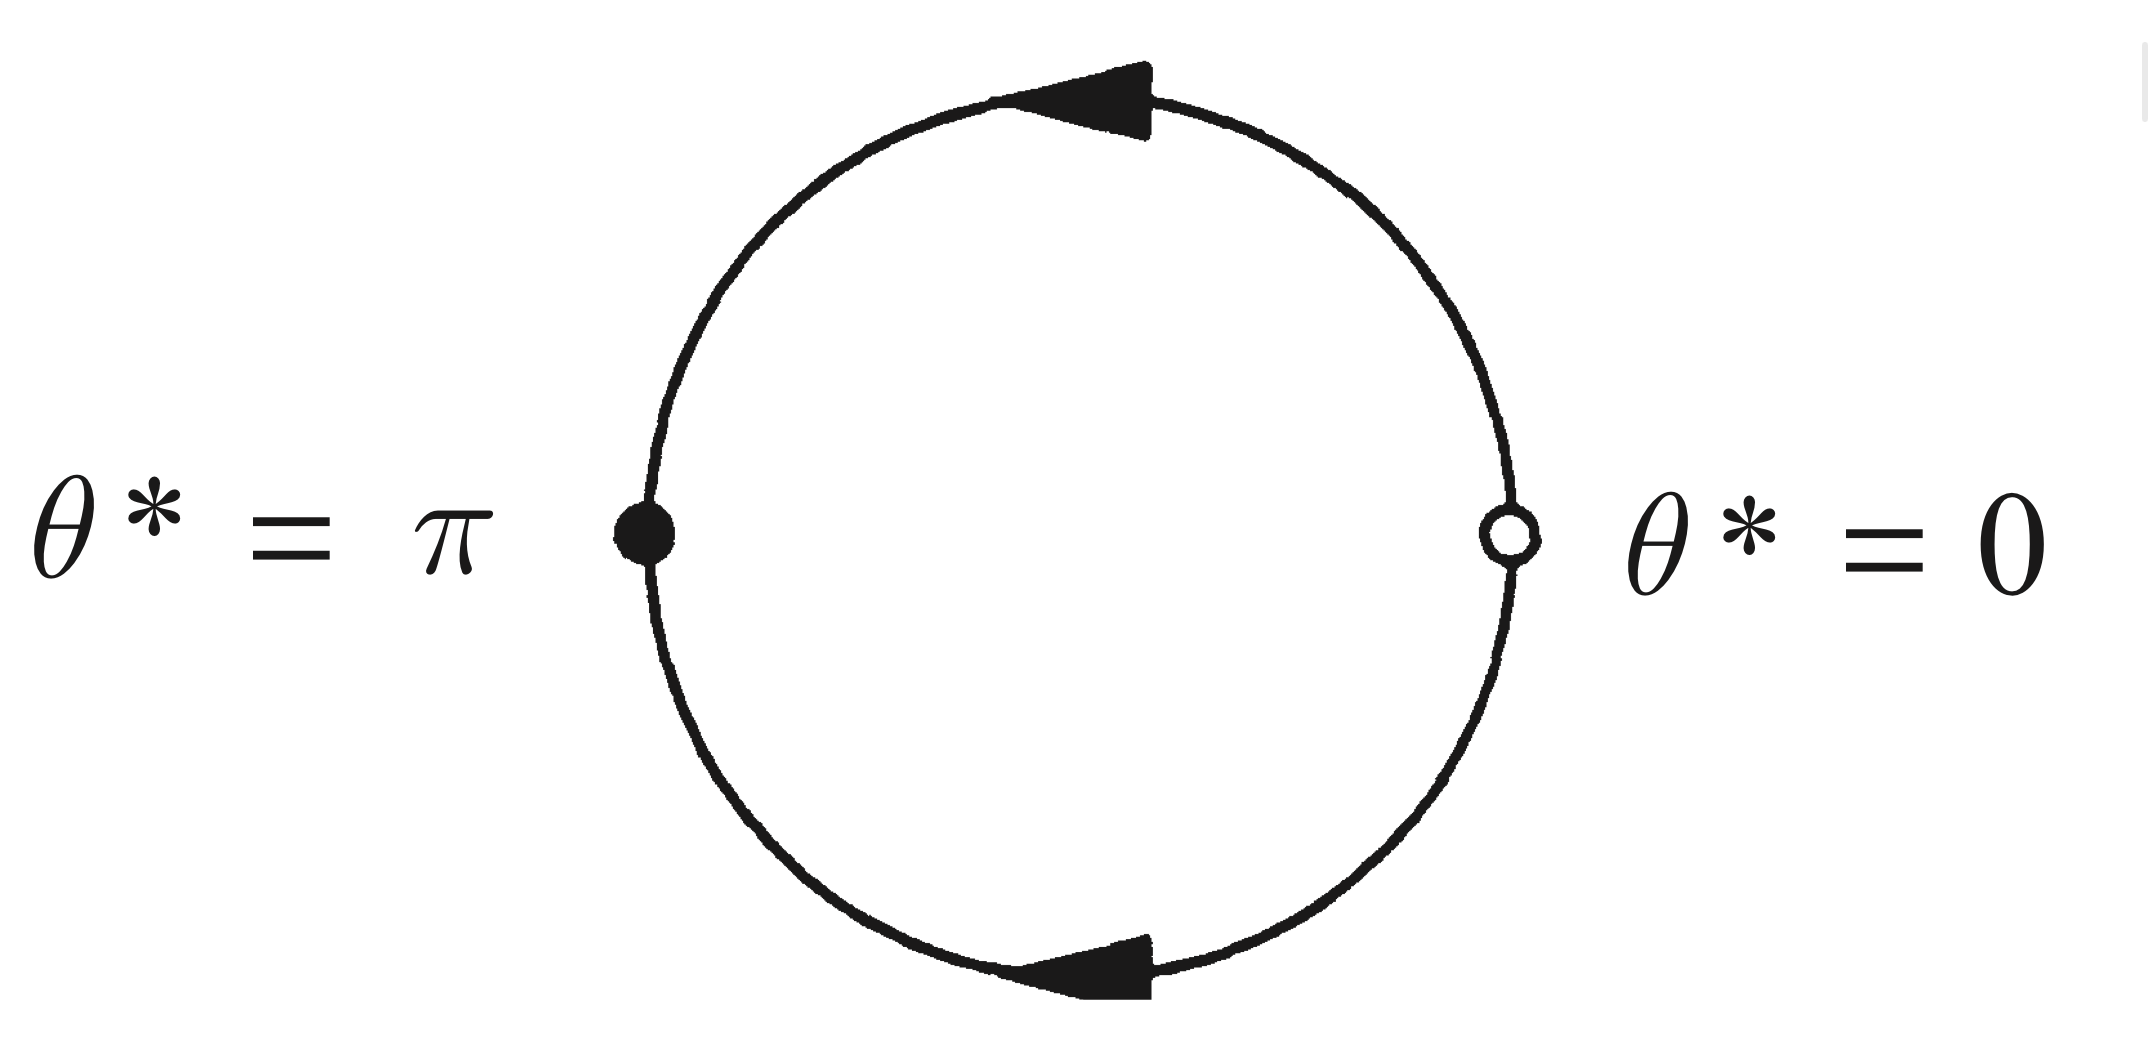
\includegraphics[width=.2\textwidth]{img/theta0.png}
\end{figure}
The function $f$ here must satisfy the condition $f(\theta+2\pi)=f(\theta)$ for all real $\theta$, and we assume as usual that $f(\theta)$ is smooth enough to guarantee existence and uniqueness of solutions. 
\section{Uniform oscillator}   
The most simple oscillator is 
\begin{equation}
    \dot \theta = \omega
\end{equation}
\section{Nonuniform oscillator}
An example of nonuniform oscillator is 
\begin{equation}
    \dot \theta = \omega - a\sin \theta, \qquad \omega >0, \alpha \ge 0
\end{equation}
\begin{figure}[H]
    \centering
    \begin{subfigure}[b]{.5\textwidth}
        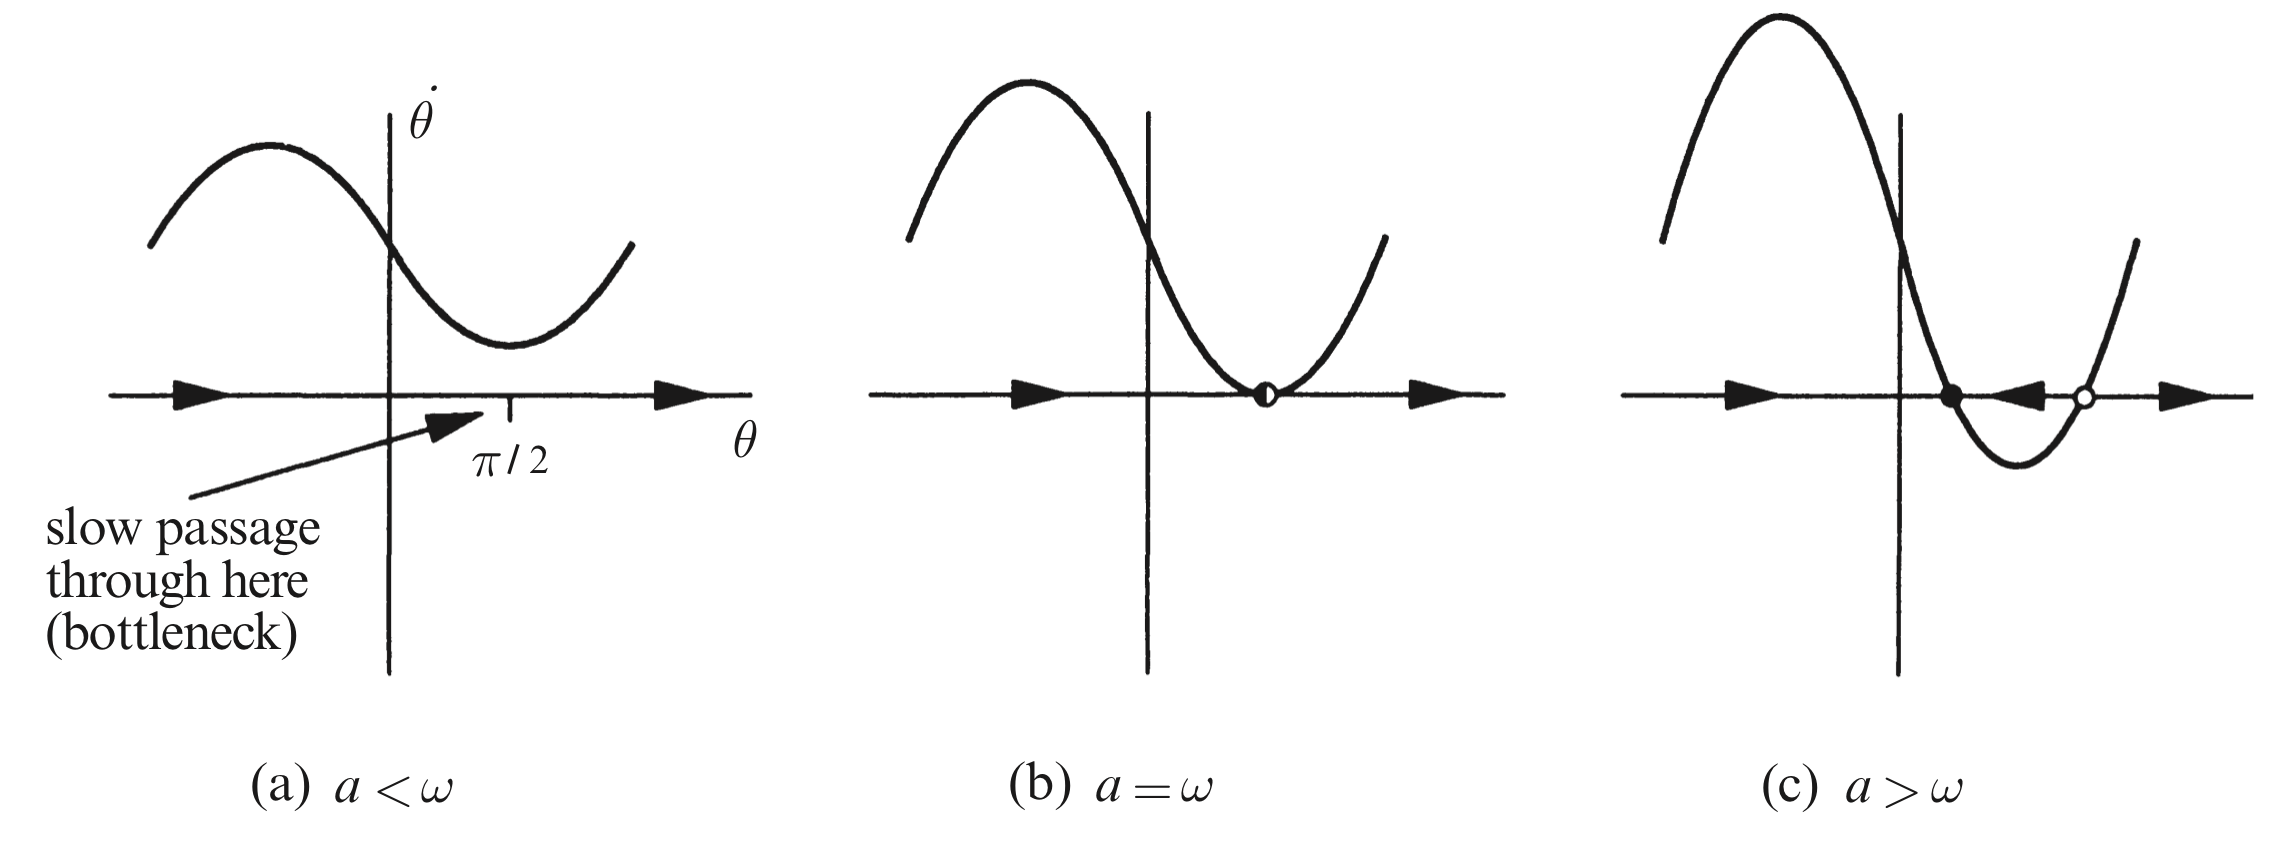
\includegraphics[width=\textwidth]{img/sin.png}
    \end{subfigure}
    \begin{subfigure}[b]{.5\textwidth}
        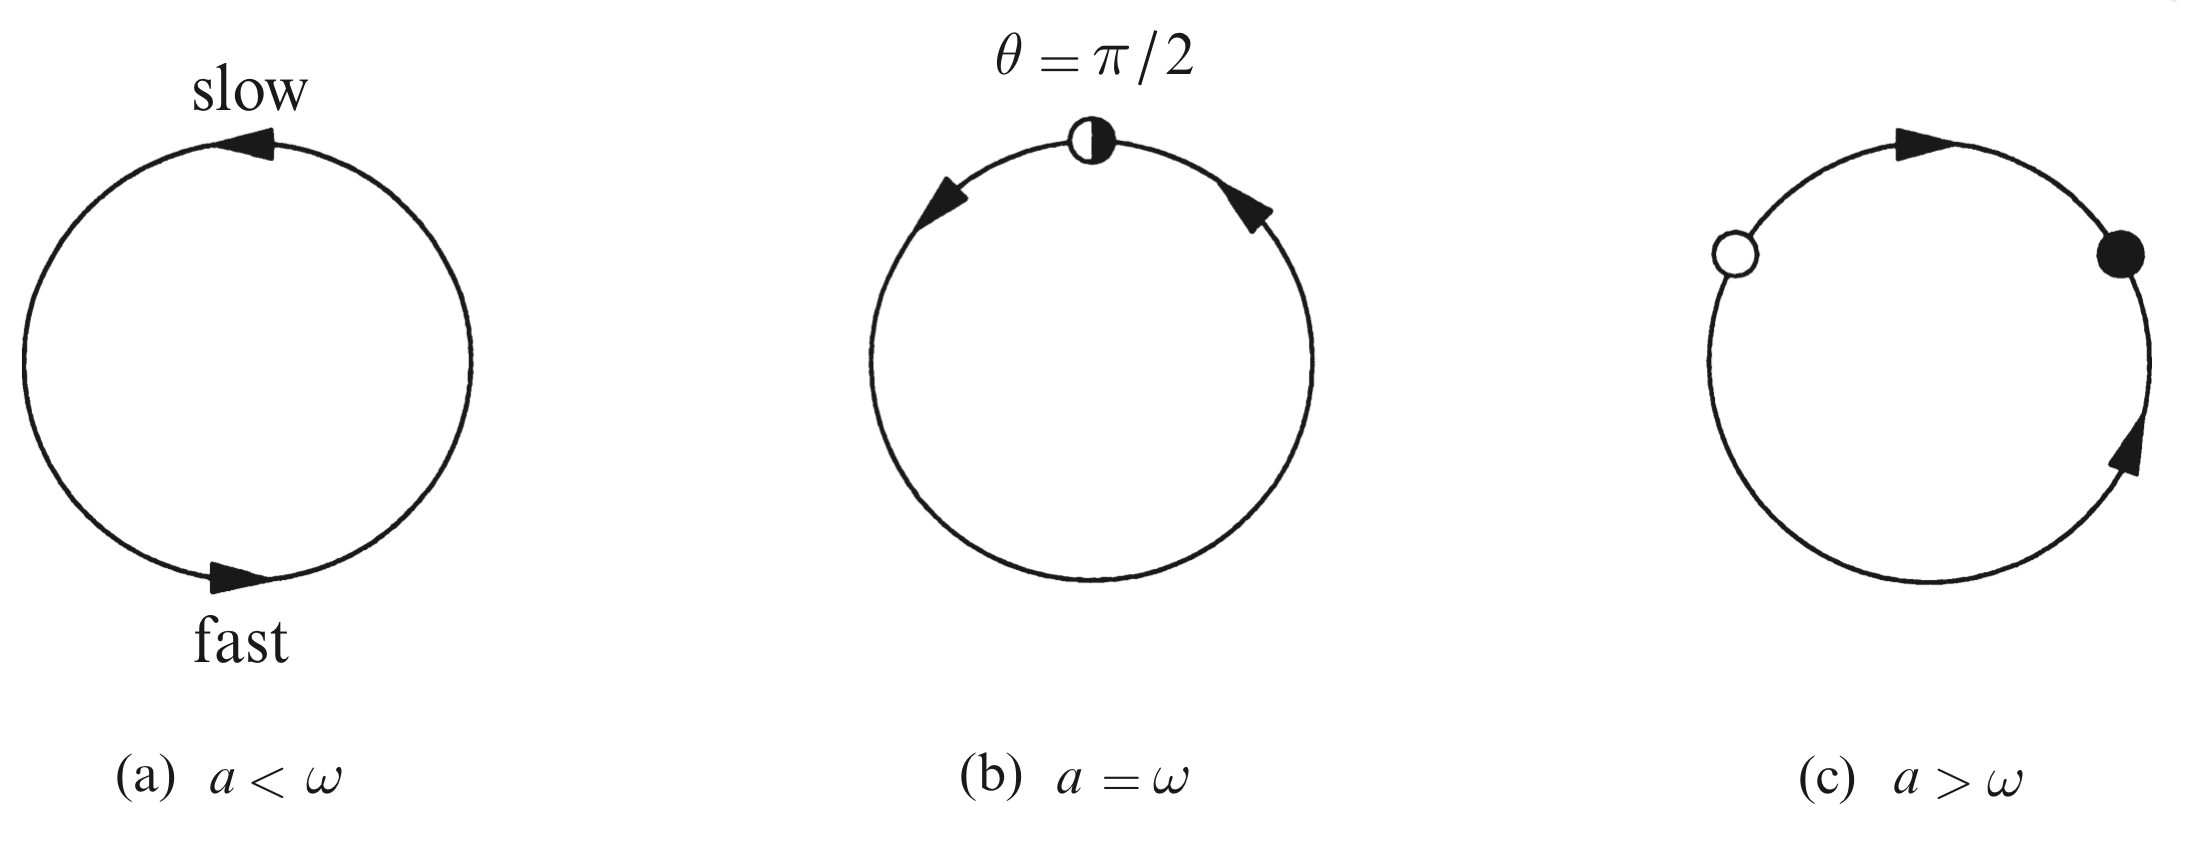
\includegraphics[width=\textwidth]{img/sin_2.png}
    \end{subfigure}
\end{figure}
\section{Fireflies}
We study here the behaviour of fireflies emitting light based on a stimulus artificial light. Suppose that $\theta(t)$ is the phase of the firefly's flashing rhythm, where $\theta = 0$ corresponds to the instant when a flash is emitted. In absence of stimuli, the firefly has a frequency $\dot \theta = \omega$. Suppose that the artificial stimulus has a phase $\Theta$ and a constant frequency $\Omega$: $\dot \Theta = \Omega$, where $\Theta=0$ corresponds to the flash of the stimulus. \\
The model of the problem of the synchronisation of the fly with the stimulus is 
\begin{equation}
    \dot \theta = \omega + A\sin (\Theta-\theta)\qquad A>0
\end{equation}
$A$ being the resetting strength, it measures the fly's ability to modify its instantaneous frequency. Introducing $\phi \coloneqq \Theta-\theta$, 
\begin{equation}
    \dot \phi = \Omega-\omega -A\sin \phi
\end{equation}
Adimensionally: 
\begin{equation}
    \phi'=\frac{d\phi}{d\tau}=\mu-\sin \phi \qquad \begin{cases}
        \tau = At\\
        \mu = \frac{\Omega-\omega}{A}
    \end{cases}
\end{equation}
\begin{figure}[H]
    \centering
    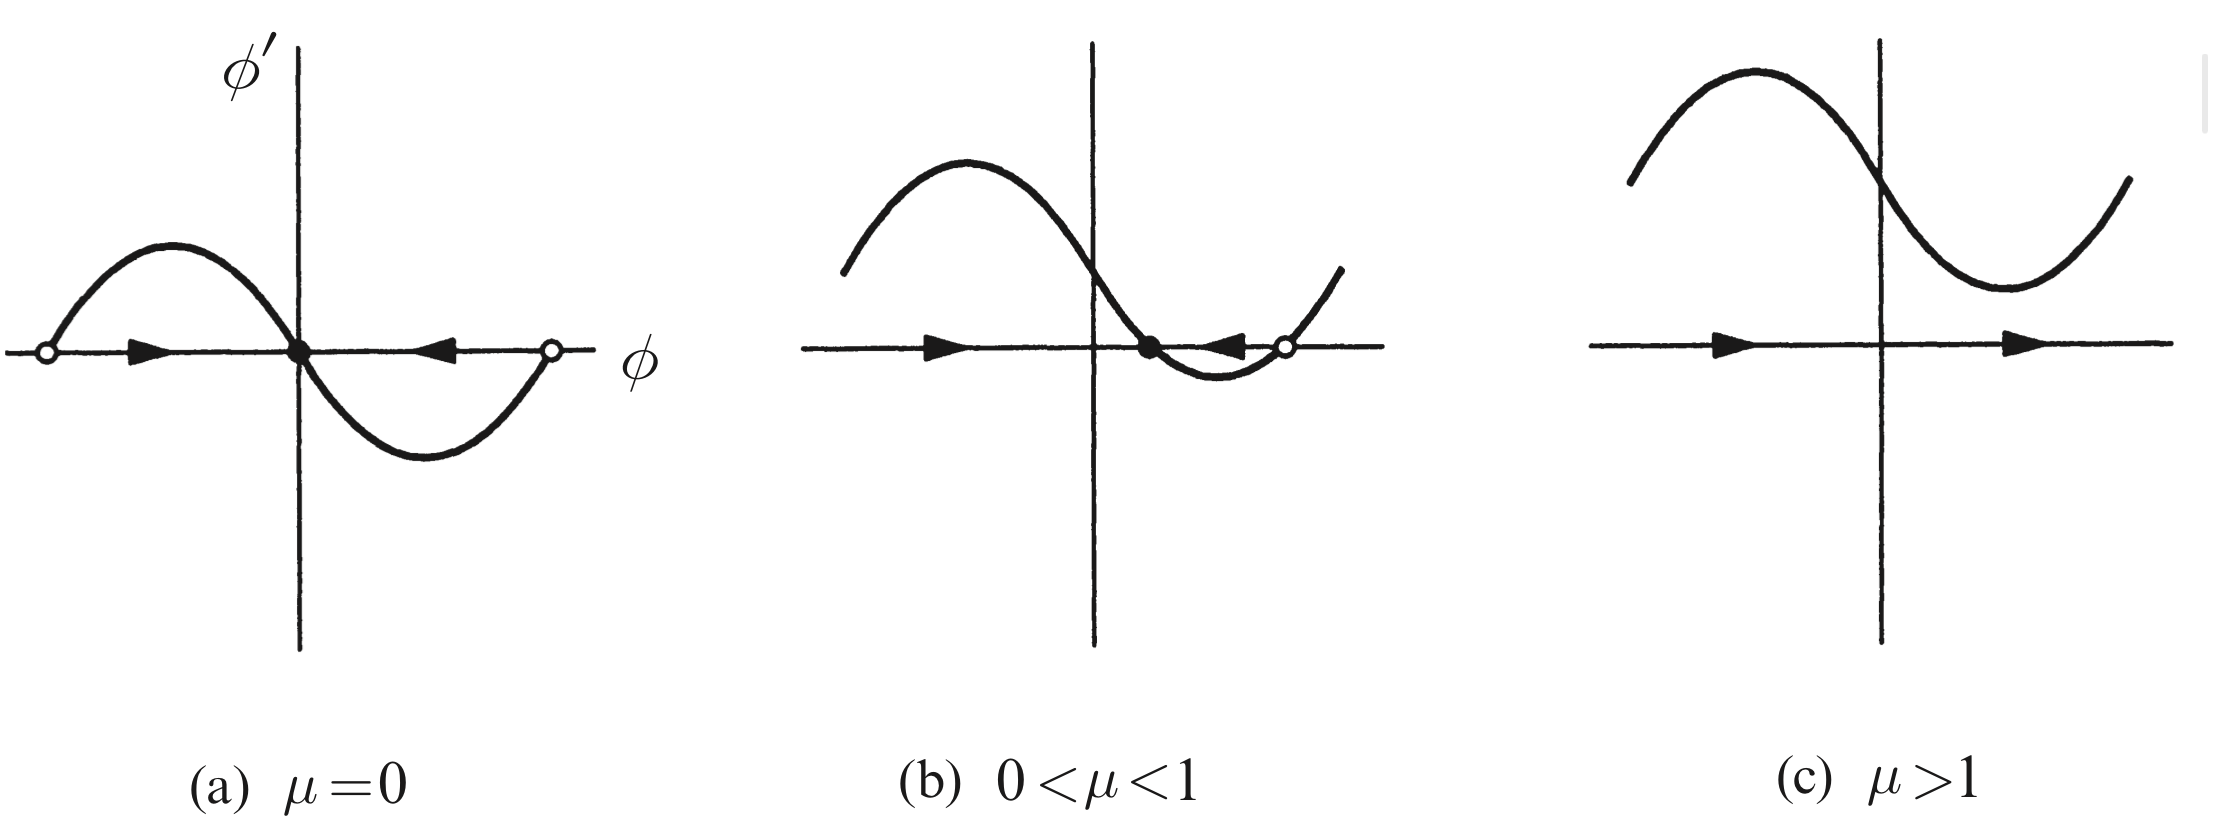
\includegraphics[width=.5\textwidth]{img/fly.png}
\end{figure}
\begin{itemize}
    \item For $\mu=0$, there is a single fixed point at $\phi^*=0$. This means that the fly and the stimulus flash simultaneously if the fly is driven at its natural frequency.
    \item For $0<\mu<1$, all trajectories are still attracted to a stable fixed point, but $\phi^*>0$. The fly's rhythm is phase-locked ot the stimulus. It means that the fly and the stimulus run with the same instantaneous frequency, although they no longer flash in unison. 
    \item For $\mu>1$, the stable and unstable points coalesce in a saddle-node biffurcation at $\mu=1$. 
\end{itemize}
\end{document}